\documentclass[preprint, 3p,
authoryear]{elsarticle} %review=doublespace preprint=single 5p=2 column
%%% Begin My package additions %%%%%%%%%%%%%%%%%%%

\usepackage[hyphens]{url}

  \journal{Transport Geography?} % Sets Journal name

\usepackage{graphicx}
%%%%%%%%%%%%%%%% end my additions to header

\usepackage[T1]{fontenc}
\usepackage{lmodern}
\usepackage{amssymb,amsmath}
% TODO: Currently lineno needs to be loaded after amsmath because of conflict
% https://github.com/latex-lineno/lineno/issues/5
\usepackage{lineno} % add
\usepackage{ifxetex,ifluatex}
\usepackage{fixltx2e} % provides \textsubscript
% use upquote if available, for straight quotes in verbatim environments
\IfFileExists{upquote.sty}{\usepackage{upquote}}{}
\ifnum 0\ifxetex 1\fi\ifluatex 1\fi=0 % if pdftex
  \usepackage[utf8]{inputenc}
\else % if luatex or xelatex
  \usepackage{fontspec}
  \ifxetex
    \usepackage{xltxtra,xunicode}
  \fi
  \defaultfontfeatures{Mapping=tex-text,Scale=MatchLowercase}
  \newcommand{\euro}{€}
\fi
% use microtype if available
\IfFileExists{microtype.sty}{\usepackage{microtype}}{}
\usepackage[]{natbib}
\bibliographystyle{plainnat}

\usepackage{graphicx}
\ifxetex
  \usepackage[setpagesize=false, % page size defined by xetex
              unicode=false, % unicode breaks when used with xetex
              xetex]{hyperref}
\else
  \usepackage[unicode=true]{hyperref}
\fi
\hypersetup{breaklinks=true,
            bookmarks=true,
            pdfauthor={},
            pdftitle={Leveraging GTFS to explore spatial gaps in transit supply with respect to social needs},
            colorlinks=false,
            urlcolor=blue,
            linkcolor=magenta,
            pdfborder={0 0 0}}

\setcounter{secnumdepth}{5}
% Pandoc toggle for numbering sections (defaults to be off)


% tightlist command for lists without linebreak
\providecommand{\tightlist}{%
  \setlength{\itemsep}{0pt}\setlength{\parskip}{0pt}}

% From pandoc table feature
\usepackage{longtable,booktabs,array}
\usepackage{calc} % for calculating minipage widths
% Correct order of tables after \paragraph or \subparagraph
\usepackage{etoolbox}
\makeatletter
\patchcmd\longtable{\par}{\if@noskipsec\mbox{}\fi\par}{}{}
\makeatother
% Allow footnotes in longtable head/foot
\IfFileExists{footnotehyper.sty}{\usepackage{footnotehyper}}{\usepackage{footnote}}
\makesavenoteenv{longtable}



\usepackage{subfig}
\usepackage{booktabs}
\usepackage{longtable}
\usepackage{array}
\usepackage{multirow}
\usepackage{wrapfig}
\usepackage{float}
\usepackage{colortbl}
\usepackage{pdflscape}
\usepackage{tabu}
\usepackage{threeparttable}
\usepackage{threeparttablex}
\usepackage[normalem]{ulem}
\usepackage{makecell}
\usepackage{xcolor}



\begin{document}


\begin{frontmatter}

  \title{Leveraging GTFS to explore spatial gaps in transit supply with
respect to social needs}
    \author[Public Transport Research Group (PTRG)]{James Reynolds%
  %
  \fnref{1}}
   \ead{james.reynolds@monash.edu} 
    \author[Public Transport Research Group (PTRG)]{Graham Currie%
  \corref{cor1}%
  \fnref{2}}
   \ead{graham.currie@monash.edu} 
    \author[Public Transport Research Group (PTRG)]{Yanda Qu%
  %
  \fnref{3}}
   \ead{yanda.qu@monash.edu} 
      \affiliation[Public Transport Research Group (PTRG)]{
    organization={Public Transport Research Group (PTRG), Institute of
Transport Studies, Department of Civil Engineering Engineering, Monash
University},addressline={Clayton
Campus},city={Melbourne},postcode={3800},state={Victoria},country={Australia},}
    \cortext[cor1]{Corresponding author}
    \fntext[1]{Research Fellow}
    \fntext[2]{Professor}
    \fntext[3]{PhD Student}
  
  \begin{abstract}
  This is the abstract.

  It consists of two paragraphs.
  \end{abstract}
    \begin{keyword}
    keyword1 \sep 
    keyword2
  \end{keyword}
  
 \end{frontmatter}

\hypertarget{introduction}{%
\section{Introduction}\label{introduction}}

A need to provide at least some motorised mobility for those who cannot
otherwise drive themselves influences transit service levels in many
places \citep{Currie:2016aa}. Age, disability, socio-economic status,
lack of a driver's license or vehicle, and many other factors might make
someone reliant on transit services for some or all of their travel.
Social-equity perspectives on transport policy-making, especially the
desire to improve vertical equity so as to better support those who are
disadvantaged (c.f. \citet{Litman:2016aa}), might therefore suggest
providing at least some transit, and probably more than just a minimum,
to places that have the highest social need for transport.

\citet{Currie2003Hobart}, \citet{Currie2004Gap},
\citet{Currie2007Identifying} and \citet{currie2010identifying}
developed an approach for identifying spatial gaps in transit supply
related to social needs for transport. This involves identifying areas
with very high needs for transport, yet little or no service, and was
applied to a case study of 2006 transit service levels in Greater
Melbourne, Australia. However, there does not appear to have been much
further use or development of this approach. As well, it is unclear if
the spatial patterns identified in this previous research, are
representative of transit supply and social needs in other places, or
whether the location of gaps in Melbourne itself have changed in the
intervening years. This may in part be because until recently transit
schedule data was not readily available in consistent, electronic
formats, meaning that assessing transit supply was a large task.

Nowadays, more than 10,000 transit agencies publicly release timetable
data in the General Transit Feed Specification (GTFS) format
\citep{GTFS}. Such standardisation allows Google Maps and other online
platforms to provide outputs for any place with a GTFS feed, and has
facilitated research and other analysis of transit services. However,
tools for using GTFS data to examine spatial patterns and gaps in
transit supply with respect to social needs for transport do not appear
to be readily available. This gap, and the lack of direct follow up to
\citet{Currie2003Hobart}, \citet{Currie2004Gap},
\citet{Currie2007Identifying} and \citet{currie2010identifying}, provide
the motivation for this paper.

The three main objectives of this research are: (1) to develop tools for
undertaking needs-gap analysis using GTFS datasets; (2) to explore
whether such gaps in Melbourne have changed since the publication of
\citet{Currie2007Identifying} and \citet{currie2010identifying}; and (3)
to better understand whether spatial patterns in Melbourne are
representative of those in other places. Research outcomes that are
reported in this paper include the development of a new R package
(gtfssupplyindex) with software tools that facilitate the use of the
\citet{Currie2003Hobart}, \citet{Currie2004Gap},
\citet{Currie2007Identifying} and \citet{currie2010identifying}
approach, in particular the calculation of transit Supply Index (SI)
scores from GTFS datasets. Also presented in this paper are results for
Australian cities in 2016 and 2021, matching the most recent censuses,
which are compared across locations and to the 2006 analysis of
Melbourne reported in \citet{currie2010identifying}.

The remainder of this paper is structured as follows: the next section
outlines the background to this research. Section 3 describes the study
methodology, followed by presentation of results in Section 4 and
discussion in Section 5. Limitations of this study, directions for
future research and a brief conclusion are provided in Section 6.

\hypertarget{research-context}{%
\section{Research context}\label{research-context}}

\hypertarget{transit-metrics}{%
\subsection{Transit metrics}\label{transit-metrics}}

There are many metrics available for benchmarking transit services.
These include those in the Transit Cooperative Research Program (TCRP)
Report 88, a guidebook for developing performance-measurement systems
\citep{Ryus:2003aa}; and those used across benchmarking databases and
programs such as \citet{Florida-Transit-Information-System:2018aa},
\citet{UITP:2015aa} and \citet{Imperial-College-London:2023aa}. The
Fielding Triangle \citep{FieldingGordonJ1987Mpts} provides a framework
for combining indicators of service inputs, outputs and consumption to
describe cost efficiency, cost effectiveness and service effectiveness.
More broadly: \citet{Litman:2003ab} and \citet{Litman:2016aa} discuss
some of the traffic, mobility, accessibility, social equity, strategic
planning and other rational decision-making-based perspectives
underlying many transport indicators; \citet{Reynolds:2017ah} extends
these into models of how institutionalism, incrementalism and other
public policy analysis concepts might apply to decision-making processes
relating to transit prioritization; \citet{GuzmanLuisA.2017Aeit}
developed a measure of accessibility in the context of policy
development and social equity for Latin American Bus Rapid Transit (BRT)
networks; and \citet{Creutzig2020streetspaceallocation} introduced
street space allocation metrics based around ten ethical principles.

However, many of these metrics may be difficult to calculate, explain or
understand, especially for those who are not planners, engineers or
other technical specialists. Where pre-calculated transit metrics are
immediately available, such as on a website or other online platform, it
may not be possible to independently generate scores, for instance to
assess proposed system changes. Contrasting examples are provided by:

\begin{itemize}
\item
  Transit Scores \citep{WalkScore:2023tg}, which are readily available
  online for locations with a published GTFS feed. The meaning of the
  metric appears easy to explain, with the highest possible score of 100
  representing the sort of transit accessibility experienced in the
  center of New York. However, the Transit Score algorithm is secret,
  and scores cannot be calculated independently or generated for
  proposed changes to networks.
\item
  The Transit Capacity and Quality of Service Manual (TCQSM), which
  provides a wide range of metrics for measuring different aspects of a
  transit system. The TCQSM scores themselves appear easy to understand
  or explain, ranging from A (good) to F (bad), although the large
  number of metrics might be somewhat overwhelming for some users. The
  scores, however, can be calculated independently, given sufficient
  data.
\end{itemize}

The widespread availability of GTFS datasets in recent years has
facilitated the development of tools, such as the Transit Score, that
apply the same metric to many transit systems. \citet{Wong:2013aa}
provides an example of what can be done with GTFS data, open metrics and
coding, by reporting the distribution of various TCQSM metrics across 50
USA transit operators. Code used in the \citet{Wong:2013aa} analysis is
available for those who might wish to produce a similar study for other
locations and systems. Developing a similar code base, but for
calculating metrics associated with spatial gaps in transit supply based
on social needs, is the subject of this paper.

\hypertarget{the-transit-suppy-index}{%
\subsection{The Transit Suppy Index}\label{the-transit-suppy-index}}

An objective of this study is to produce code that facilitates
calculation of the SI metric from GTFS data. A generalized form of the
SI equation, adapted from \citet{currie2010identifying}, is:

\[SI_{area, time} = \sum{\frac{Area_{Bn}}{Area_{area}}SL_{n, time}}\]

where:

\begin{itemize}
\item
  \(SI_{area, time}\) is the Supply Index for the area of interest and a
  given period of time;
\item
  \(Area_{Bn}\) is the buffer area for each stop (n) within the area of
  interest (in \citet{currie2010identifying} this was based on a radius
  of 400 metres for bus and tram stops, and 800 metres for railway
  stations);
\item
  \(Area_{area}\) is the area of the area of interest; and
\item
  \(SL_{n,time}\) is the number of transit arrivals for each stop for a
  given time period.
\end{itemize}

\begin{figure}
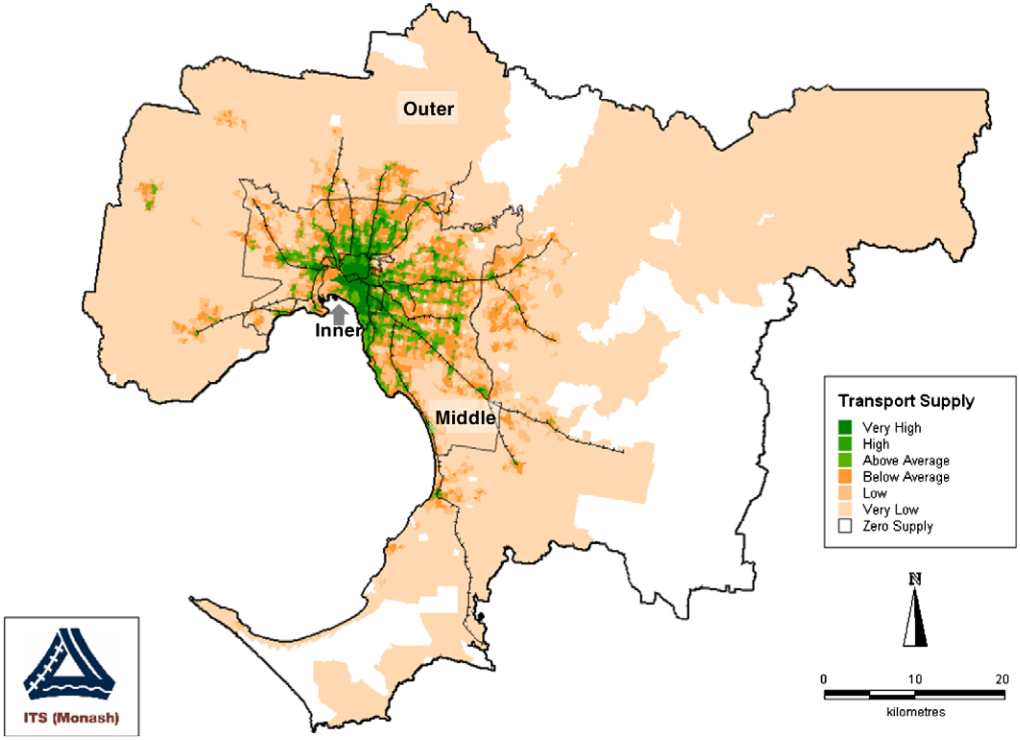
\includegraphics[width=1\linewidth]{graphics/Currie2010SI} \caption{Distribution of supply measure scores – Metropolitan Melbourne (2006), Source: Currie (2010)}\label{fig:Currie_map_SI}
\end{figure}

\citet{currie2010identifying} reported SI scores for Census Collection
Districts (CCDs) across Metropolitan Melbourne in 2006, as shown in
Figure \ref{fig:Currie_map_SI}. General patterns were identified, being:
more transit supply in the middle and inner suburbs, and along passenger
railway lines; and outer areas tending to have very low SI scores or no
transit supply at all.

\hypertarget{social-need-and-needs-gap}{%
\subsection{Social need and needs-gap}\label{social-need-and-needs-gap}}

As well as measuring transit supply, \citet{currie2010identifying}
assessed the social need for transport across Metropolitan Melbourne
using: the Australian Bureaus of Statistics' Index of Related
Socio-Economic Advantage/Disadvantage (IRSAD) and a transport needs
index derived from eight weighted indicators. The spatial distribution
of this composite social needs index in 2006, reproduced in Figure
\textbackslash ref\{fig:Currie\_map\_needs), showed that areas of above
average, high and very high social needs in 2006 were located in: some
outer areas, particularly in the east and south-east; and in some middle
areas in the south-east, north and west.

\begin{figure}
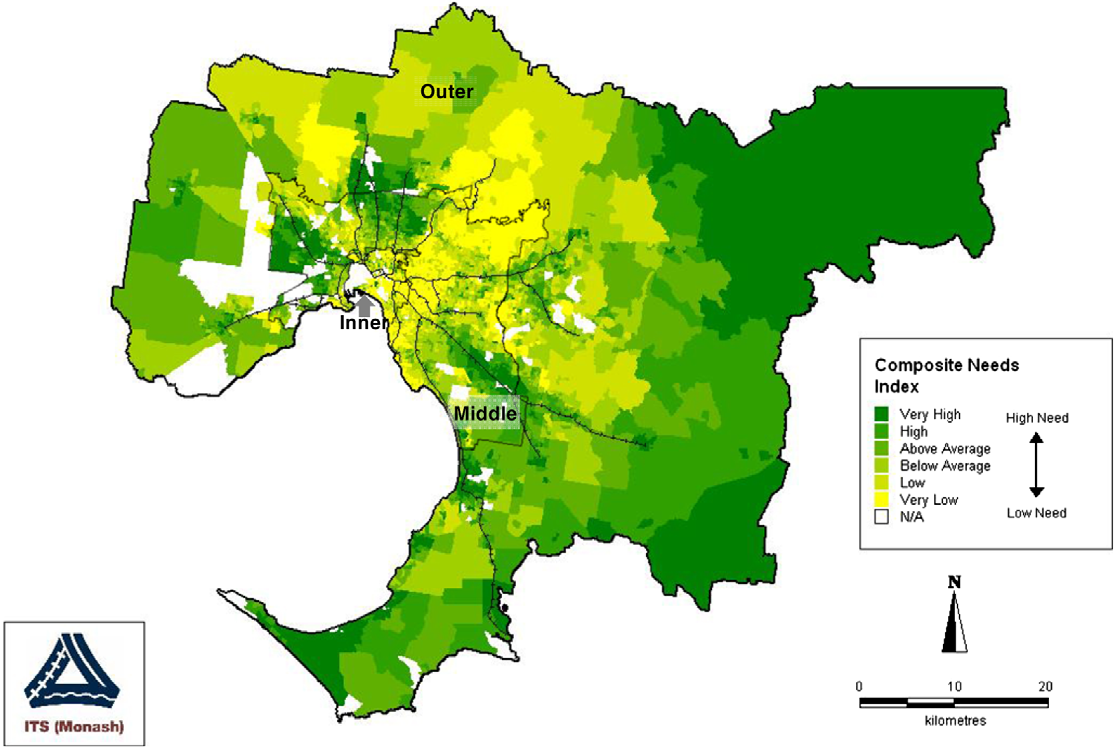
\includegraphics[width=1\linewidth]{graphics/Currie2010Needs} \caption{Distribution of categories of composite social need index scores - Metropolitan Melbourne (2006). Source: Currie (2010.)}\label{fig:Currie_map_needs}
\end{figure}

As the final step in the spatial needs-gap analysis,
\citet{currie2010identifying} identified areas with very high transport
needs, but very low or no transit supply, as reproduced in Figure
\ref{fig:Currie_map_gap}. These areas were identified as being those
where service gaps might be of particular concern. Most of these were
located in outer parts of Melbourne in the north-east, south-east and
south, although there were also some pockets in the middle suburbs in
the west, north and south east. Overall, \citet{currie2010identifying}
found that ``8.2\% of Melbourne residents have `very high' needs but
`zero', `low' or `very low' public transport supply.''

\begin{figure}
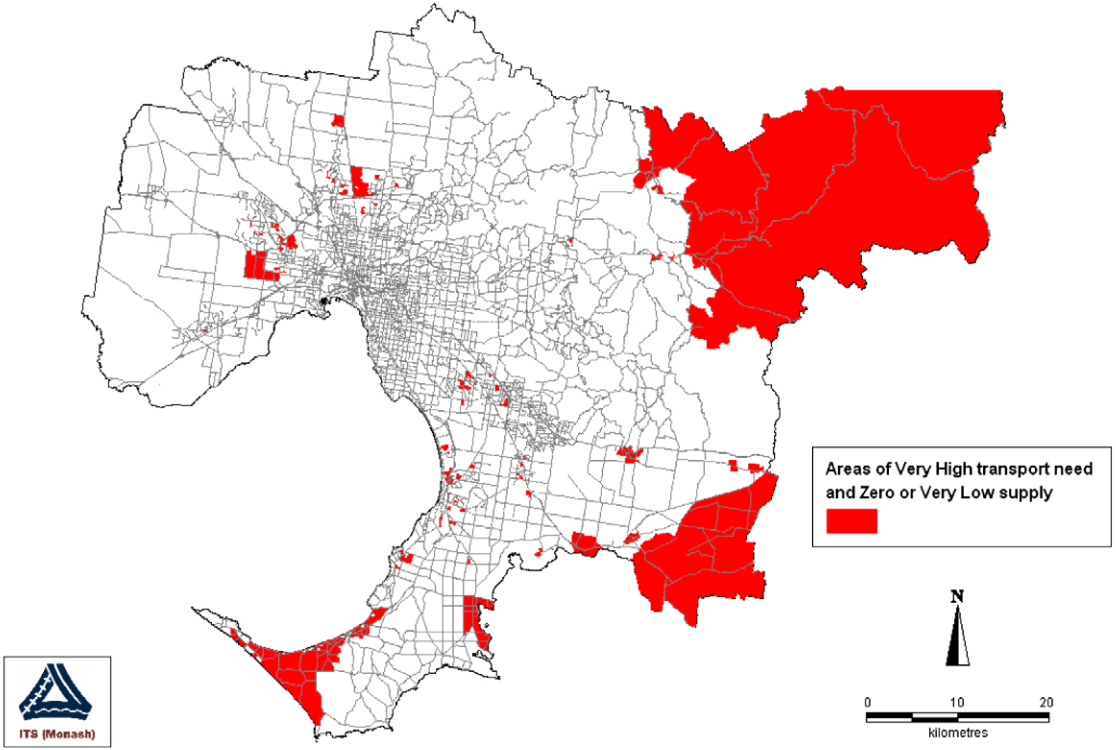
\includegraphics[width=1\linewidth]{graphics/Currie2010gap} \caption{Distribution of CCDs with very high transport needs and with zero or very low public transport supply - Metropolitan Melbourne (2006). Source: Currie (2010)}\label{fig:Currie_map_gap}
\end{figure}

Using this methodology in transit planning was suggested as
``substantially more useful than the presentation of anecdotal evidence,
which is the most common means of identifying transport needs in local
transport studies throughout the world''\citep{currie2010identifying}.
However, it does not appear that this approach has been widely adopted
in practice or by researchers. Our suspicion is that while the SI has a
relatively simple formula and requires only geographic and timetable
data to calculate, a lack of software tools may be partly why it has not
been more widely adopted.

It is also unclear whether the patterns in Melbourne identified in
\citet{currie2010identifying} have changed since the 2006 analysis, or
if Melbourne is representative of other locations. Developing a software
tool to calculate SI tools from GTFS data, and then using it to
comparing current conditions and other locations to the findings of
\citet{currie2010identifying}, therefore, provides the motivation for
this research.

\hypertarget{methodology}{%
\section{Methodology}\label{methodology}}

\hypertarget{code-development}{%
\subsection{Code development}\label{code-development}}

This study developed a package of tools for calculating the SI from GTFS
data using the R programming language \citep{R-base}. The
recommendations of \citet{wickham2023r} informed the package setup and
development approach. Various existing packages and code examples were
relied upon including: the sf package \citep{R-sf} for geospatial
analysis; the tidyverse \citep{tidyverse2019}; gtfstools
\citep{R-gtfstools}; and tidytransit \citep{R-tidytransit}. Australian
Bureau of Statistics (ABS) data was also used, sourced via the strayr
and absmapsdata packages \citep{r-strayr}.

Code was developed and tested on the Mornington Peninsula Tourist
Railway GTFS feed. This was selected primarily for convenience, given
that the authors are familiar with the surrounding geography and that
the feed covers a small number of trips across just three stations.

\hypertarget{changes-since-2006-in-melbourne}{%
\subsection{Changes since 2006 in
Melbourne}\label{changes-since-2006-in-melbourne}}

Much has changed since 2006, including the spatial geography used by the
Australian Bureau of Statistics (ABS) to collect census data. To allow
direct comparison between 2006 and the most recent census, therefore,
this study calculated SI scores using the same Census Collection
Districts (CCDs) used by \citet{currie2010identifying} for the week
starting the day of the 2021 census. The Victorian GTFS feed, published
by Public Transport Victoria (PTV), was used with historical feeds
sourced via \citet{transitfeeds_victoria:2023aa}.

Unfortunately, it is not possible to obtain 2016 or 2021 social
disadvantage data for CCDs, as the ABS no longer releases data using
this geographic scheme. Instead, population and other statistics are now
released for Statistical Area 1 (SA1) zones, which have been adopted as
the areas-of-interest in this study.

\hypertarget{variation-in-spatial-patterns-across-location-and-time.}{%
\subsection{Variation in spatial patterns across location and
time.}\label{variation-in-spatial-patterns-across-location-and-time.}}

SI scores were also calculated for other capital cities in Australia,
for the weeks starting on the days of the 2016 and 2021 censuses.
Historical GTFS data was again sourced via the Transit Feeds website.
Unfortunately it was not possible to locate 2021 GTFS data for Greater
Sydney or Greater Darwin, so SI scores were calculated for 2024 using
the latest data sets, sourced directly from the relevant transit
authorities.

\hypertarget{measuring-social-disadvantage}{%
\subsection{Measuring social
disadvantage}\label{measuring-social-disadvantage}}

This study adopts a similar approach to measuring social disadvantage as
used in \citet{currie2010identifying}, using: the ABS' Index of Relative
Socio-Economic Advantage/Disadvantage (IRSAD); and a transport needs
index\footnote{The same need indicators and weightings used in
  \citet{currie2010identifying} were adopted, although \$799 or lower
  per week was used as the threshold for low income households rather
  than \$499 to account for inflation (as per the Reserve Bank of
  Australia's online inflation calculator).}. A composite needs
indicator was derived based on the IRSAD and the transport needs index,
again as per the \citet{currie2010identifying} approach. However,
changes to the ABS reporting systems mean that the composite needs
indicator had to be based on weighting both the IRSAD index and the
transport need index by the total population of each SA1 zone, which
were then added, standardised and split into six groups\footnote{This
  contrasts to the method used by \citet{currie2010identifying}, where
  the composite needs index also included relative need components,
  being the IRSAD and the transport needs indexes weighted by the
  population within the various needs groups in each area of interest
  (for a total of four indicators included in the composite needs
  indicator, compared to only two in the 2016 and 2021 results presented
  here.}.

\hypertarget{results}{%
\section{Results}\label{results}}

\hypertarget{the-gtfssupplyindex-package}{%
\subsection{The gtfssupplyindex
Package}\label{the-gtfssupplyindex-package}}

Code developed to calculate SI scores is available as an R package on
github (see \citet{gtfssupplyindex_github}). Included in the package is
a vignette (INCLUDE LINK) that outlines the structure of the
calculations, the developed functions. Also included in the vignette are
step-by-step calculations for the Mornington Peninsula Railway as a
worked example, and comparison to SI scores calculated manually.

\hypertarget{melbourne}{%
\subsection{Melbourne}\label{melbourne}}

\hypertarget{transport-supply-categories}{%
\subsubsection{Transport Supply
Categories}\label{transport-supply-categories}}

\begin{figure}
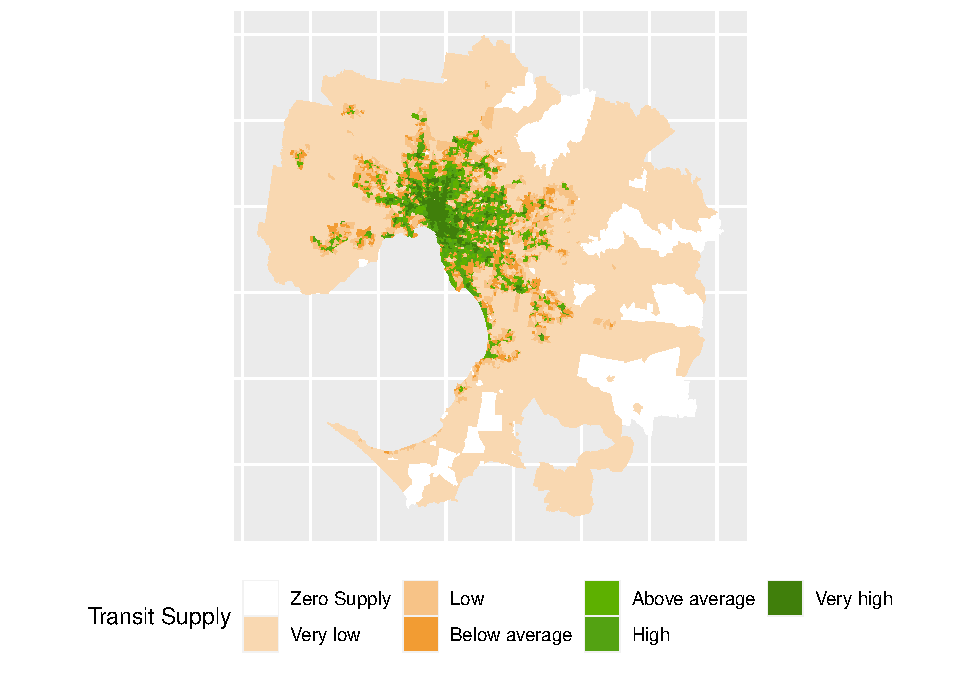
\includegraphics[width=1\linewidth]{Leveraging_GTFS_to_assess_transit_supply_Transport_Geography_files/figure-latex/Greater_Melbourne_CCD_2021-1} \caption{Melbourne (2006 extents), Transport Supply by CCD, week starting the day of the 2016 (left) and 2021 (right) censuses}\label{fig:Greater_Melbourne_CCD_2021}
\end{figure}

\begin{figure}
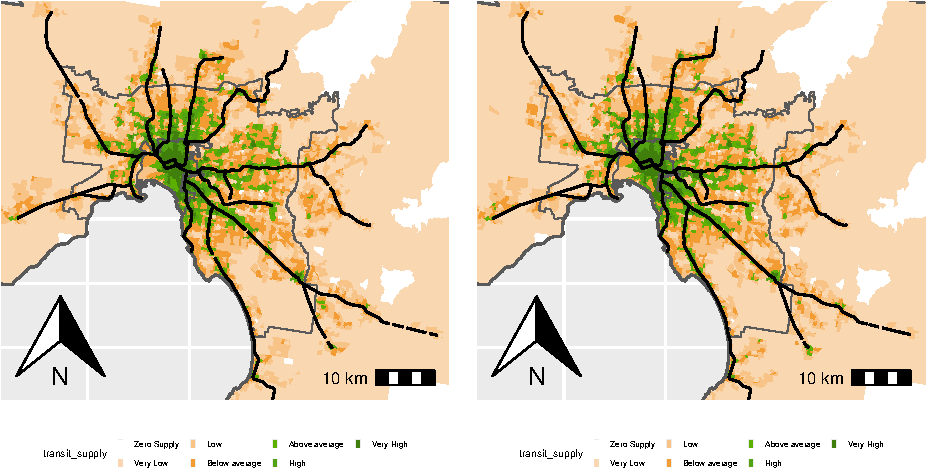
\includegraphics[width=1\linewidth]{Leveraging_GTFS_to_assess_transit_supply_Transport_Geography_files/figure-latex/Greater_Melbourne_CCD_2021_rail_extents-1} \caption{Melbourne, extent of suburban rail network (except Stony Point line)), Transport Supply by CCD, week starting the day of the 2016 (left) and 2021 (right) censuses}\label{fig:Greater_Melbourne_CCD_2021_rail_extents}
\end{figure}

Figures \ref{fig:Greater_Melbourne_CCD_2021} shows the distribution of
Transport Supply categories\footnote{The same Transport Supply
  categorizations have been used as in \citet{currie2010identifying},
  with those CCDs that have above average SI scores split evenly into
  three groups, those that have below average SIs also split evenly into
  three groups, and those CCDs without SI scores of zero placed in their
  own category. Hence, both Figure \ref{fig:Currie_map_SI} and Figure
  \ref{fig:Greater_Melbourne_CCD_2021} show relative service levels in
  each CCD compared to the rest of Greater Melbourne for that year.}
across Melbourne in the weeks of the 2016 and 2021 censuses, using the
same (2006) CCD boundaries\footnote{Note, however, that there are some
  inconsistencies in the CCDs included in Metropolitan Melbourne in
  \citet{currie2010identifying} (5,839) and the number included in ABS
  dataset used for this analysis (6,325).} as in Figure
\ref{fig:Currie_map_SI}. Figure
\ref{fig:Greater_Melbourne_CCD_2021_rail_extents} shows the same data,
but at a higher scale so as to zoom in on parts of Melbourne within the
extents of the suburban rail network.

The overall spatial patterns appear generally similar in 2016 and 2021
as they were in 2006, with higher levels of transit supply in inner
areas and close to most railway lines. However, clear differences
include:

\begin{itemize}
\tightlist
\item
  areas in the outer west (around Melton) that had above average supply
  in 2006 had below average supply in 2016 and 2021.
\item
  some middle south-eastern suburbs along the bay (vicinty of Black
  Rock) and outer eastern suburbs (Ferntree Gully) have dropped below
  average, while a small area in the middle to outer south has moved
  from being below average in 2006 to above average in 2016 (Kananook,
  immediately north of Frankston) and 2021 (Kananook and Bonbeach).
\item
  there have been suburban railway extensions to the north-west
  (Sunbury) and north-east (to South Morang in 2013 and to Mernda in
  2018). The former involved electrification to incorporate existing
  line segments (already served by country services) into the surburban
  network. Transport Supply to Sunbury, however, appears to still be
  below average, suggesting that not much has changed following the
  shift from service by regional trains to suburban trains. For Mernda
  in contrast, there has been increases in service levels, with some
  areas now having Above Average supply.
\item
  Some areas, away from railway lines, have also shifted from below
  average supply in 2006 to above average supplies in 2016 and 2021,
  including in the middle north-west (Greenvale) and middle to outer
  south east (Narre Warren South).
\item
  Services appear to have been introduced to some outer eastern (east of
  Gembrook), south-eastern (Koo Wee Rup, Lang Lang, Nar Nar Goon,
  Garfield, Bunyip and others) and southern (St Andrews Beach) areas.
\end{itemize}

\begin{figure}
\centering
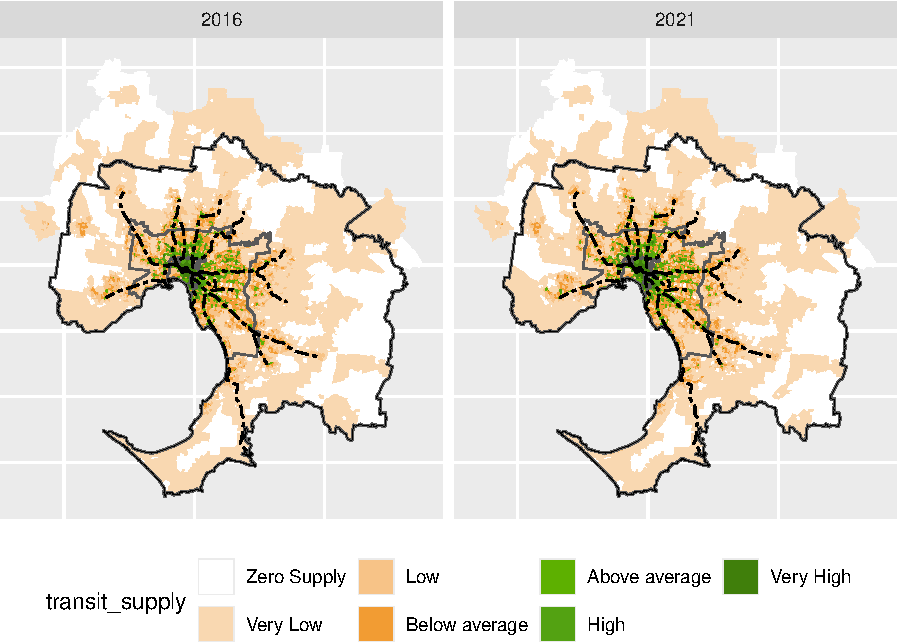
\includegraphics{Leveraging_GTFS_to_assess_transit_supply_Transport_Geography_files/figure-latex/Greater_Melbourne_2016_2021_plot-1.pdf}
\caption{Greater Melbourne, Transit Supply by SA1 for the weeks starting
the date of 2016 and 2021 census, overlayed with: 2006 Greater Melbourne
boundary (black); 2021 SA4 boundaries (grey); and suburban railway lines
(dashed)}
\end{figure}

\begin{figure}
\centering
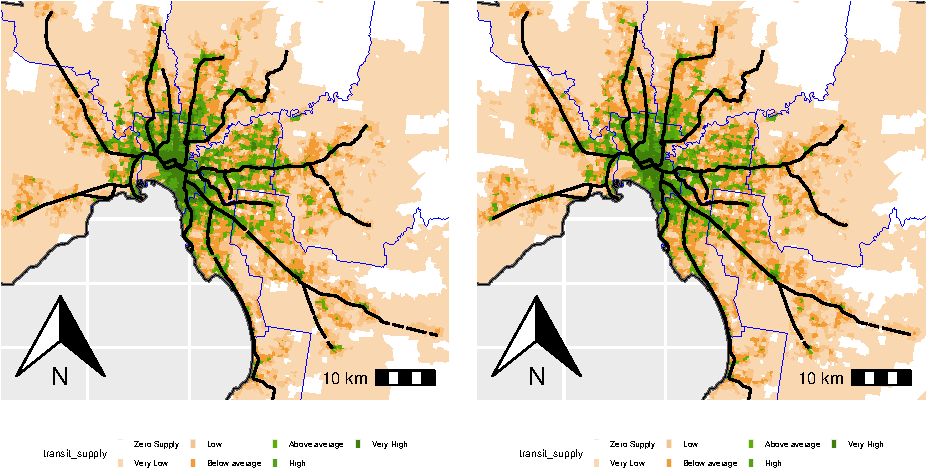
\includegraphics{Leveraging_GTFS_to_assess_transit_supply_Transport_Geography_files/figure-latex/Greater_Melbourne_2016_2021_plot_railway_extents-1.pdf}
\caption{Greater Melbourne (extents of suburban railway network),
Transit Supply by SA1 for the weeks starting the date of 2016 and 2021
census, overlayed with: 2021 SA4 boundaries (grey); and suburban railway
lines (dashed)}
\end{figure}

\begin{longtable}[t]{lrrrrr}
\caption{\label{tab:Greater_Melbourne_CCDs_SA1_table}Distribution of 2006, 2016 and 2021 Transport Supply to Melbourne CCDs (2006 boundaries), 2016 Transport Supply to Greater Melbourne (2016 SA1s) and 2021 Transport Supply to Greater Melbourne (2021 SA1s). Sources: 2006 values, Currie (2010); 2016 and 2021 values, authors' analysis}\\
\toprule
\multicolumn{1}{c}{Transport} & \multicolumn{3}{c}{CCDs} & \multicolumn{1}{c}{2016 SA1s} & \multicolumn{1}{c}{2021 SA1s} \\
\cmidrule(l{3pt}r{3pt}){1-1} \cmidrule(l{3pt}r{3pt}){2-4} \cmidrule(l{3pt}r{3pt}){5-5} \cmidrule(l{3pt}r{3pt}){6-6}
Supply & 2006 & 2016 & 2021 & 2016 & 2021\\
\midrule
Zero Supply & 3.2\%   (189) & 1.4\%    (86) & 1.3\%    (81) & 3.2\%    (326) & 4.3\%    (489)\\
Very Low & 22.5\% (1,314) & 23.5\% (1,485) & 23.3\% (1,474) & 23.0\%  (2,362) & 23.4\%  (2,692)\\
Low & 22.4\% (1,310) & 23.5\% (1,484) & 23.3\% (1,473) & 23.0\%  (2,362) & 23.4\%  (2,691)\\
Below average & 22.2\% (1,294) & 23.5\% (1,484) & 23.3\% (1,473) & 23.0\%  (2,362) & 23.4\%  (2,691)\\
Above average & 10.4\%   (608) & 9.4\%   (596) & 9.6\%   (608) & 9.3\%    (959) & 8.5\%    (975)\\
\addlinespace
High & 9.2\%   (535) & 9.4\%   (595) & 9.6\%   (608) & 9.3\%    (959) & 8.5\%    (974)\\
Very High & 10.1\%   (589) & 9.4\%   (595) & 9.6\%   (608) & 9.3\%    (959) & 8.5\%    (975)\\
Total & 100.0\% (5,839) & 100.0\% (6,325) & 100.0\% (6,325) & 100.0\% (10,289) & 100.0\% (11,487)\\
\bottomrule
\end{longtable}

\begin{figure}
\centering
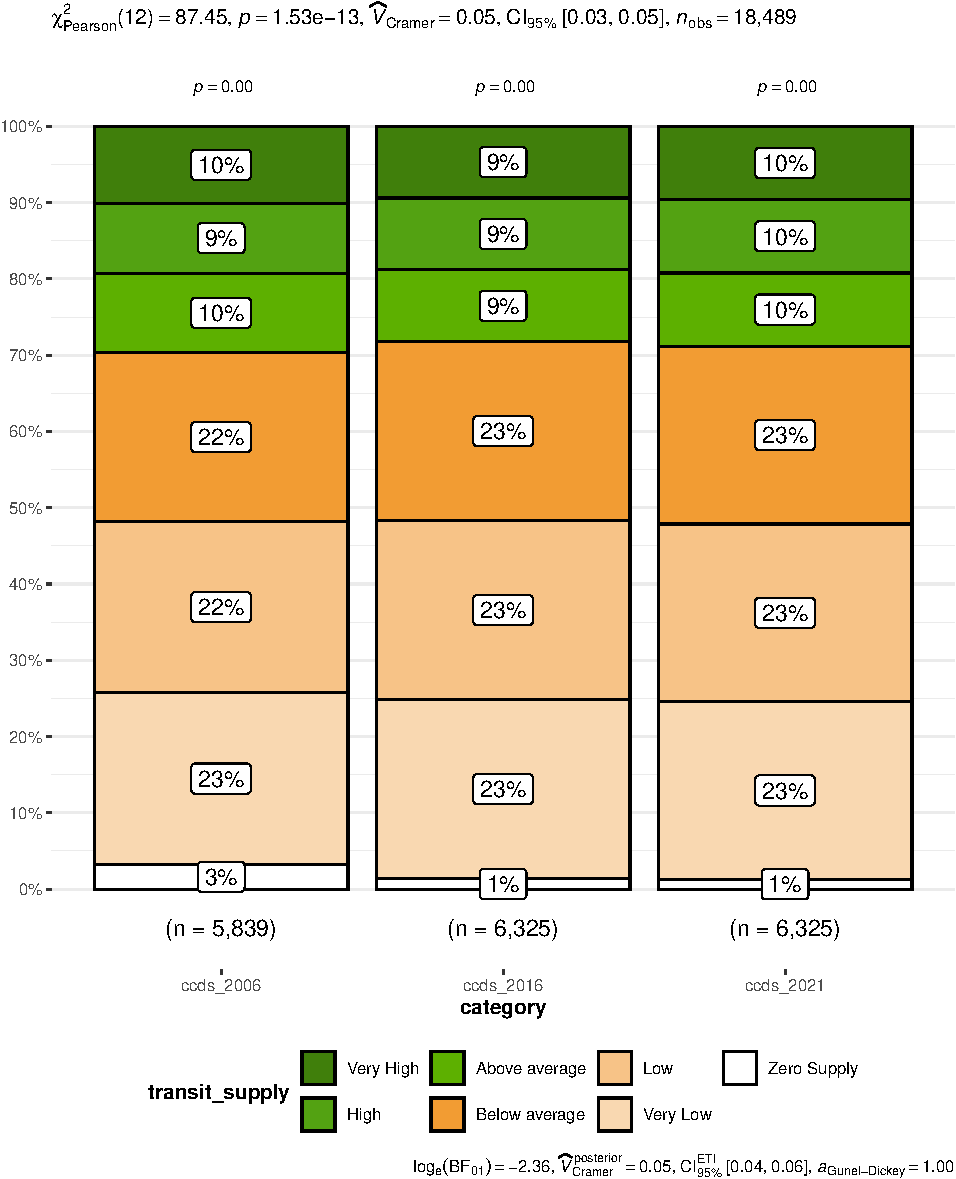
\includegraphics{Leveraging_GTFS_to_assess_transit_supply_Transport_Geography_files/figure-latex/Greater_Melbourne_CCDs_SA1_table-1.pdf}
\caption{Distribution of 2006, 2016 and 2021 Transit Supply to 2006
CCDs. Sources: 2006 values - Currie (2010), 2016 and 2021 values -
authors}
\end{figure}

\begin{figure}
\centering
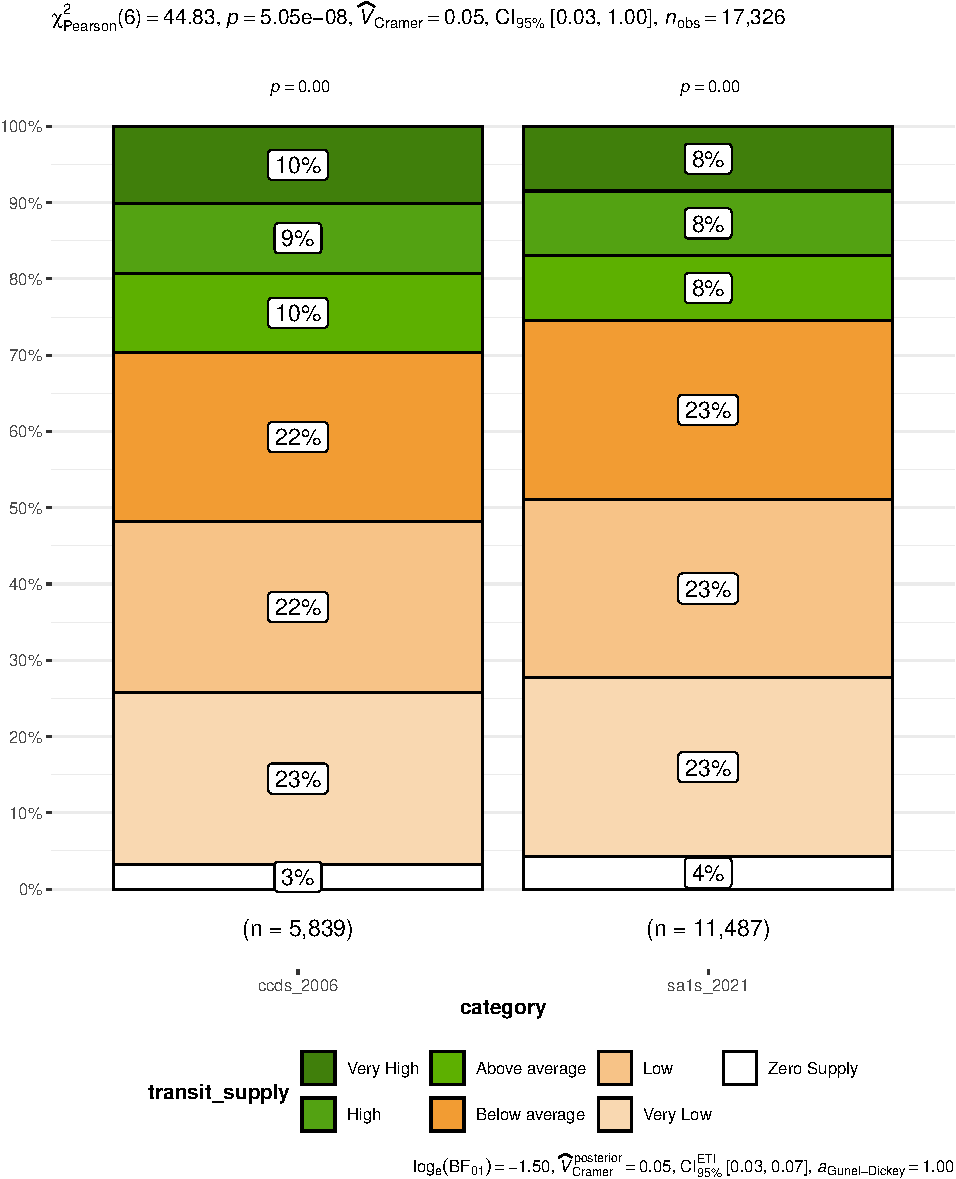
\includegraphics{Leveraging_GTFS_to_assess_transit_supply_Transport_Geography_files/figure-latex/Greater_Melbourne_SA1s_bar_stats-1.pdf}
\caption{Distribution of Transit Supply to 2006 CCDs, 2021 CCDs and 2021
SA1s, population 2006 and 2021. Sources: 2006 values - Currie (2010),
2021 values - authors}
\end{figure}

Table \ref{tab:Greater_Melbourne_SA1_2021_table} summarises the
distribution of CCDs and SA1s across different Transport Supply
categories in 2006, 2016 and 2021. Figure
\ref{fig:Greater_Melbourne_CCDs_SA1_table} compares the shares of CCDs
in each category in 2006, 2016 and 2021, for which differences are
statistically significant (\(\chi^2(12, N = 18489) = 87.45\),
\(p < .001\)), with only 81 in 2021 (1.3\%) of the CCDs in Melbourne
having Zero Supply in 2021, compared to the 189 (3.2\%) reported by
\citet{currie2010identifying} for 2006. Differences are also
statistically significant when comparing each pair separately (2006 vs
2016, \(\chi^2(6, N = 12164) = 56.87\), \(p < .001\); 2006 vs 2021
\(\chi^2(6, N = 12164) = 59.15\), \(p < .001\); and 2016 vs 2021
\(\chi^2(6, N = 12650) = 0.67\), \(p = .995\)).

These values, however, are for CCDs within the 2006 extents of
Melbourne. The ABS' statistical boundary of ``Greater Melbourne'' now
includes areas up to around 30 kilometers further to the north of the
2006 boundary, as shown in Figures
\ref{fig:Greater_Melbourne_2016_2021_plot} and
\ref{fig:Greater_Melbourne_2016_2021_plot_railway_extents}. These
figures indicate that the new parts of Melbourne, beyond the 2006
statistical boundary, generally have Very Low or Zero Transport Supply
levels. There are many minor differences between the 2016 and 2021
spatial distributions, but the overall patterns remain generally
similar. The fifth and sixth columns in Table
\ref{tab:Greater_Melbourne_SA1_2021_table} report the distribution of
Transport Supply category across all of Greater Melbourne, adopting the
2016 and 2021 SA1 zones. Again, the differences between 2006 (CCDs),
2016 and 2021 (SA1s) are statistically significant
(\(\chi^2(12, N = 27615) = 58.86\), \(p < .001\)) as are the difference
when comparing each pair (2006 vs 2016, \(\chi^2(6, N = 16128) = 8.83\),
\(p = .183\); 2006 vs 2021 \(\chi^2(6, N = 17326) = 44.83\),
\(p < .001\); and 2016 vs 2021 \(\chi^2(6, N = 21776) = 31.56\),
\(p < .001\)). There are a greater proportion of SA1s with Zero Supply
in 2021 (4.3\%) than there were CCDs in 2006. The share of SA1s with
supply below the average (i.e.~Zero, Very Low, Low or Below Average) is
also larger in 2021 (74.5\%) compared to the share of CCDs in 2006
(70.3\%).

\begin{longtable}[]{@{}
  >{\raggedright\arraybackslash}p{(\columnwidth - 6\tabcolsep) * \real{0.1972}}
  >{\raggedleft\arraybackslash}p{(\columnwidth - 6\tabcolsep) * \real{0.2676}}
  >{\raggedleft\arraybackslash}p{(\columnwidth - 6\tabcolsep) * \real{0.2676}}
  >{\raggedleft\arraybackslash}p{(\columnwidth - 6\tabcolsep) * \real{0.2676}}@{}}
\caption{Distribution of 2006, 2016 and 2021 Transport Supply to
population in Melbourne. Sources: 2006 values, Currie (2010); 2016 and
2021 values, authors' analysis}\tabularnewline
\toprule\noalign{}
\begin{minipage}[b]{\linewidth}\raggedright
Supply
\end{minipage} & \begin{minipage}[b]{\linewidth}\raggedleft
2006
\end{minipage} & \begin{minipage}[b]{\linewidth}\raggedleft
2016
\end{minipage} & \begin{minipage}[b]{\linewidth}\raggedleft
2021
\end{minipage} \\
\midrule\noalign{}
\endfirsthead
\toprule\noalign{}
\begin{minipage}[b]{\linewidth}\raggedright
Supply
\end{minipage} & \begin{minipage}[b]{\linewidth}\raggedleft
2006
\end{minipage} & \begin{minipage}[b]{\linewidth}\raggedleft
2016
\end{minipage} & \begin{minipage}[b]{\linewidth}\raggedleft
2021
\end{minipage} \\
\midrule\noalign{}
\endhead
\bottomrule\noalign{}
\endlastfoot
Zero Supply & 2.5\% (85,423) & 2.9\% (131,619) & 3.8\% (186,829) \\
Very Low & 23.6\% (793,046) & 22.5\% (1,008,498) & 23.0\% (1,132,967) \\
Low & 25.7\% (865,330) & 22.7\% (1,016,848) & 23.7\% (1,163,358) \\
Below average & 23.0\% (774,521) & 22.3\% (1,000,290) & 23.6\%
(1,159,783) \\
Above average & 9.6\% (324,546) & 9.3\% (418,614) & 8.7\% (426,892) \\
High & 7.7\% (260,411) & 9.6\% (428,880) & 8.7\% (425,779) \\
Very High & 7.8\% (263,832) & 10.7\% (480,469) & 8.6\% (422,025) \\
Total & 100.0\% (3,367,109) & 100.0\% (4,485,218) & 100.0\%
(4,917,633) \\
\end{longtable}

\begin{figure}
\centering
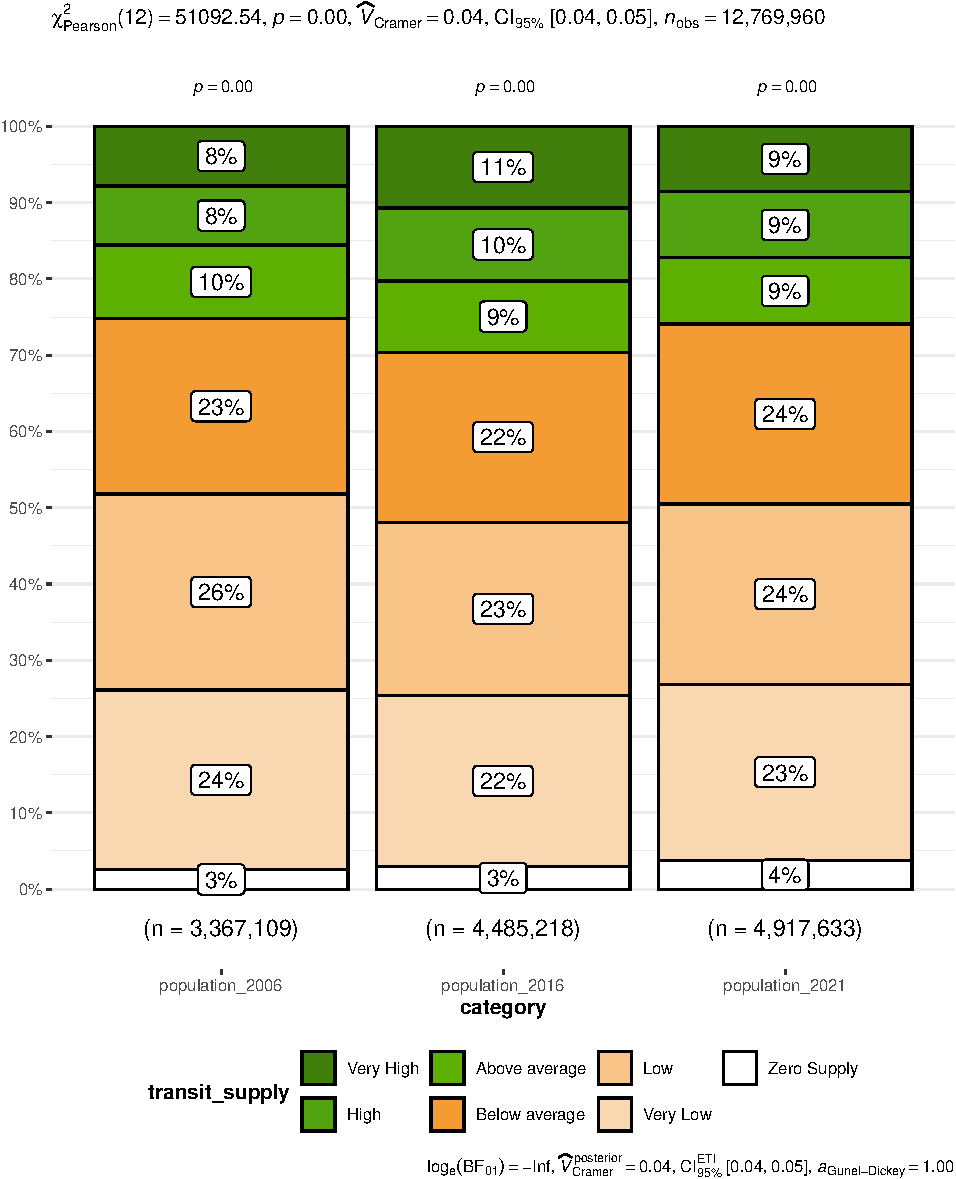
\includegraphics{Leveraging_GTFS_to_assess_transit_supply_Transport_Geography_files/figure-latex/Greater_Melbourne_CCDs_SA1_population-1.pdf}
\caption{Distribution of Transit Supply to population in 2006 (CCDs),
2016 and 2021 (SA1s). Sources: 2006 values - Currie (2010), 2021 values
- authors}
\end{figure}

Table \ref{tab:Greater_Melbourne_CCDs_SA1_population} and Figure
\ref{fig:Greater_Melbourne_CCDs_SA1_population} compare the share of
resident population in each transport supply category. Differences are
statistically significant across 2006 and 2021
(\(\chi^2(6, N = 8284742) = 19038.97\), \(p < .001\)). The number of
people with zero supply rose from 85,423 (2.5\%) in 2006 to 186,829
(3.8\%) in 2021. This represents a 118.7\% increase, compared to the
population increase of 46.0\% across all of Greater Melbourne. The
number of people with zero or very low supply rose from 878,469 (26.1\%)
in 2006 to 1,319,796 (26.8\%) in 2021. This represents a 50.2\%
increase. The number of people with a supply that was below the average
(Zero, Very Low, Low or Below Average) rose from 2,518,320 (74.8\%) in
2006 to 3,642,937 (74.1\%) in 2021. This represents a 44.7\% increase.

Differences were also statistically significant between 2016 and 2021
(\(\chi^2(6, N = 9402851) = 22467.17\), \(p < .001\)). The number of
people with zero supply rose from 131,619 (2.9\%) in 2016 (+55,210,
+41.9\%, compared to the population increase of 9.6\% across all of
Greater Melbourne. The number of people with zero or very low supply
rose from 1,140,117 (25.4\%) (+179,679, +15.8\%). The number of people
with a supply that was below the average (Zero, Very Low, Low or Below
Average) rose from 3,157,255 (70.4\%) in 2016 (+ 485,682, 15.4\%).

\begin{longtable}[]{@{}
  >{\raggedright\arraybackslash}p{(\columnwidth - 20\tabcolsep) * \real{0.0833}}
  >{\raggedleft\arraybackslash}p{(\columnwidth - 20\tabcolsep) * \real{0.0889}}
  >{\raggedleft\arraybackslash}p{(\columnwidth - 20\tabcolsep) * \real{0.0833}}
  >{\raggedleft\arraybackslash}p{(\columnwidth - 20\tabcolsep) * \real{0.0833}}
  >{\raggedleft\arraybackslash}p{(\columnwidth - 20\tabcolsep) * \real{0.0889}}
  >{\raggedleft\arraybackslash}p{(\columnwidth - 20\tabcolsep) * \real{0.0833}}
  >{\raggedleft\arraybackslash}p{(\columnwidth - 20\tabcolsep) * \real{0.0889}}
  >{\raggedleft\arraybackslash}p{(\columnwidth - 20\tabcolsep) * \real{0.0889}}
  >{\raggedright\arraybackslash}p{(\columnwidth - 20\tabcolsep) * \real{0.0889}}
  >{\raggedleft\arraybackslash}p{(\columnwidth - 20\tabcolsep) * \real{0.1167}}
  >{\raggedleft\arraybackslash}p{(\columnwidth - 20\tabcolsep) * \real{0.1056}}@{}}
\caption{Greater Melbourne 2016: Share of population in each Transport
Supply category for each SA4 region}\tabularnewline
\toprule\noalign{}
\begin{minipage}[b]{\linewidth}\raggedright
transit\_supply
\end{minipage} & \begin{minipage}[b]{\linewidth}\raggedleft
Inner
\end{minipage} & \begin{minipage}[b]{\linewidth}\raggedleft
Inner East
\end{minipage} & \begin{minipage}[b]{\linewidth}\raggedleft
Inner South
\end{minipage} & \begin{minipage}[b]{\linewidth}\raggedleft
North East
\end{minipage} & \begin{minipage}[b]{\linewidth}\raggedleft
North West
\end{minipage} & \begin{minipage}[b]{\linewidth}\raggedleft
Outer East
\end{minipage} & \begin{minipage}[b]{\linewidth}\raggedleft
South East
\end{minipage} & \begin{minipage}[b]{\linewidth}\raggedright
West
\end{minipage} & \begin{minipage}[b]{\linewidth}\raggedleft
Mornington Peninsula
\end{minipage} & \begin{minipage}[b]{\linewidth}\raggedleft
Total
\end{minipage} \\
\midrule\noalign{}
\endfirsthead
\toprule\noalign{}
\begin{minipage}[b]{\linewidth}\raggedright
transit\_supply
\end{minipage} & \begin{minipage}[b]{\linewidth}\raggedleft
Inner
\end{minipage} & \begin{minipage}[b]{\linewidth}\raggedleft
Inner East
\end{minipage} & \begin{minipage}[b]{\linewidth}\raggedleft
Inner South
\end{minipage} & \begin{minipage}[b]{\linewidth}\raggedleft
North East
\end{minipage} & \begin{minipage}[b]{\linewidth}\raggedleft
North West
\end{minipage} & \begin{minipage}[b]{\linewidth}\raggedleft
Outer East
\end{minipage} & \begin{minipage}[b]{\linewidth}\raggedleft
South East
\end{minipage} & \begin{minipage}[b]{\linewidth}\raggedright
West
\end{minipage} & \begin{minipage}[b]{\linewidth}\raggedleft
Mornington Peninsula
\end{minipage} & \begin{minipage}[b]{\linewidth}\raggedleft
Total
\end{minipage} \\
\midrule\noalign{}
\endhead
\bottomrule\noalign{}
\endlastfoot
Zero Supply & 0.0\% (0) & 0.0\% (480) & 0.0\% (1,604) & 0.4\% (16,988) &
0.4\% (17,655) & 0.3\% (12,955) & 1.0\% (44,757) & 0.3\% (12,056) &
0.6\% (25,124) & 2.9\% (131,619) \\
Very Low & 0.1\% (3,427) & 0.4\% (18,454) & 0.6\% (24,944) & 2.5\%
(112,269) & 2.1\% (94,853) & 4.3\% (190,890) & 4.8\% (215,217) & 4.2\%
(186,665) & 3.6\% (161,779) & 22.5\% (1,008,498) \\
Low & 0.4\% (18,018) & 0.9\% (39,235) & 1.4\% (60,833) & 2.7\% (119,608)
& 2.4\% (107,693) & 3.0\% (135,247) & 5.0\% (224,097) & 5.4\% (242,438)
& 1.6\% (69,679) & 22.7\% (1,016,848) \\
Below average & 1.0\% (42,950) & 2.3\% (105,168) & 2.9\% (128,014) &
2.9\% (132,008) & 2.2\% (97,739) & 2.7\% (119,691) & 4.0\% (177,817) &
3.8\% (170,015) & 0.6\% (26,888) & 22.3\% (1,000,290) \\
Above average & 1.0\% (44,547) & 1.8\% (80,002) & 1.8\% (81,038) & 1.0\%
(46,965) & 0.6\% (28,905) & 0.6\% (25,188) & 1.2\% (53,228) & 1.2\%
(54,895) & 0.1\% (3,846) & 9.3\% (418,614) \\
High & 2.9\% (129,533) & 1.7\% (74,966) & 1.7\% (74,617) & 1.0\%
(46,291) & 0.3\% (14,464) & 0.3\% (15,371) & 0.7\% (33,365) & 0.9\%
(38,499) & 0.0\% (1,774) & 9.6\% (428,880) \\
Very High & 7.9\% (353,232) & 0.9\% (41,416) & 0.7\% (32,561) & 0.5\%
(21,197) & 0.0\% (2,033) & 0.0\% (314) & 0.2\% (6,893) & 0.5\% (22,823)
& 0.0\% (0) & 10.7\% (480,469) \\
Total & 13.2\% (591,707) & 8.0\% (359,721) & 9.0\% (403,611) & 11.0\%
(495,326) & 8.1\% (363,342) & 11.1\% (499,656) & 16.8\% (755,374) &
16.2\% (727,391) & 6.4\% (289,090) & 100.0\% (4,485,218) \\
\end{longtable}

\begin{longtable}[]{@{}
  >{\raggedright\arraybackslash}p{(\columnwidth - 20\tabcolsep) * \real{0.0820}}
  >{\raggedleft\arraybackslash}p{(\columnwidth - 20\tabcolsep) * \real{0.0874}}
  >{\raggedleft\arraybackslash}p{(\columnwidth - 20\tabcolsep) * \real{0.0874}}
  >{\raggedleft\arraybackslash}p{(\columnwidth - 20\tabcolsep) * \real{0.0874}}
  >{\raggedleft\arraybackslash}p{(\columnwidth - 20\tabcolsep) * \real{0.0874}}
  >{\raggedleft\arraybackslash}p{(\columnwidth - 20\tabcolsep) * \real{0.0874}}
  >{\raggedleft\arraybackslash}p{(\columnwidth - 20\tabcolsep) * \real{0.0874}}
  >{\raggedleft\arraybackslash}p{(\columnwidth - 20\tabcolsep) * \real{0.0874}}
  >{\raggedright\arraybackslash}p{(\columnwidth - 20\tabcolsep) * \real{0.0874}}
  >{\raggedleft\arraybackslash}p{(\columnwidth - 20\tabcolsep) * \real{0.1148}}
  >{\raggedleft\arraybackslash}p{(\columnwidth - 20\tabcolsep) * \real{0.1038}}@{}}
\caption{Greater Melbourne 2021: Share of population in each Transport
Supply category for each SA4 region}\tabularnewline
\toprule\noalign{}
\begin{minipage}[b]{\linewidth}\raggedright
transit\_supply
\end{minipage} & \begin{minipage}[b]{\linewidth}\raggedleft
Inner
\end{minipage} & \begin{minipage}[b]{\linewidth}\raggedleft
Inner East
\end{minipage} & \begin{minipage}[b]{\linewidth}\raggedleft
Inner South
\end{minipage} & \begin{minipage}[b]{\linewidth}\raggedleft
North East
\end{minipage} & \begin{minipage}[b]{\linewidth}\raggedleft
North West
\end{minipage} & \begin{minipage}[b]{\linewidth}\raggedleft
Outer East
\end{minipage} & \begin{minipage}[b]{\linewidth}\raggedleft
South East
\end{minipage} & \begin{minipage}[b]{\linewidth}\raggedright
West
\end{minipage} & \begin{minipage}[b]{\linewidth}\raggedleft
Mornington Peninsula
\end{minipage} & \begin{minipage}[b]{\linewidth}\raggedleft
Total
\end{minipage} \\
\midrule\noalign{}
\endfirsthead
\toprule\noalign{}
\begin{minipage}[b]{\linewidth}\raggedright
transit\_supply
\end{minipage} & \begin{minipage}[b]{\linewidth}\raggedleft
Inner
\end{minipage} & \begin{minipage}[b]{\linewidth}\raggedleft
Inner East
\end{minipage} & \begin{minipage}[b]{\linewidth}\raggedleft
Inner South
\end{minipage} & \begin{minipage}[b]{\linewidth}\raggedleft
North East
\end{minipage} & \begin{minipage}[b]{\linewidth}\raggedleft
North West
\end{minipage} & \begin{minipage}[b]{\linewidth}\raggedleft
Outer East
\end{minipage} & \begin{minipage}[b]{\linewidth}\raggedleft
South East
\end{minipage} & \begin{minipage}[b]{\linewidth}\raggedright
West
\end{minipage} & \begin{minipage}[b]{\linewidth}\raggedleft
Mornington Peninsula
\end{minipage} & \begin{minipage}[b]{\linewidth}\raggedleft
Total
\end{minipage} \\
\midrule\noalign{}
\endhead
\bottomrule\noalign{}
\endlastfoot
Zero Supply & 0.0\% (0) & 0.3\% (478) & 0.9\% (1,655) & 14.2\% (26,563)
& 11.9\% (22,186) & 7.6\% (14,125) & 28.9\% (53,966) & 23.5\% (43,898) &
12.8\% (23,958) & 100.0\% (186,829) \\
Very Low & 0.4\% (4,169) & 1.8\% (20,688) & 2.0\% (22,483) & 11.5\%
(130,715) & 9.8\% (110,814) & 17.7\% (200,810) & 22.1\% (250,684) &
19.5\% (221,337) & 15.1\% (171,267) & 100.0\% (1,132,967) \\
Low & 1.7\% (20,329) & 3.9\% (45,160) & 5.5\% (63,802) & 11.3\%
(132,001) & 10.6\% (123,314) & 13.4\% (155,603) & 22.9\% (265,995) &
24.9\% (289,518) & 5.8\% (67,636) & 100.0\% (1,163,358) \\
Below average & 4.7\% (54,918) & 11.5\% (133,305) & 12.8\% (148,585) &
13.0\% (151,240) & 11.2\% (129,918) & 9.9\% (114,658) & 17.6\% (204,093)
& 15.9\% (184,466) & 3.3\% (38,600) & 100.0\% (1,159,783) \\
Above average & 13.2\% (56,422) & 16.2\% (69,199) & 21.8\% (92,875) &
10.4\% (44,470) & 6.4\% (27,140) & 5.2\% (22,262) & 12.5\% (53,328) &
13.0\% (55,438) & 1.3\% (5,758) & 100.0\% (426,892) \\
High & 35.6\% (151,439) & 17.3\% (73,687) & 16.3\% (69,281) & 10.3\%
(43,985) & 2.3\% (9,710) & 2.6\% (10,905) & 5.8\% (24,707) & 9.7\%
(41,100) & 0.2\% (965) & 100.0\% (425,779) \\
Very High & 78.1\% (329,654) & 7.3\% (30,949) & 5.7\% (23,906) & 2.8\%
(11,752) & 0.3\% (1,285) & 0.0\% (0) & 1.7\% (7,308) & 4.1\% (17,171) &
0.0\% (0) & 100.0\% (422,025) \\
Total & 12.5\% (616,931) & 7.6\% (373,466) & 8.6\% (422,587) & 11.0\%
(540,726) & 8.6\% (424,367) & 10.5\% (518,363) & 17.5\% (860,081) &
17.3\% (852,928) & 6.3\% (308,184) & 100.0\% (4,917,633) \\
\end{longtable}

Table \ref{tab:Greater_Melbourne_population_2016_by_SA4} and Table
\ref{tab:Greater_Melbourne_population_2021_by_SA4} show the distribution
of Transport Supply categories to the population in each SA4 zone in
2016 and 2021 respectively. Variations across SA4 zones are
statistically significant in both 2016
(\(\chi^2(48, N = 4485218) = 2847273.25\), \(p < .001\)) and 2021
(\(\chi^2(48, N = 4917633) = 3126013.64\), \(p < .001\)). In general,
outer areas of Greater Melbourne\footnote{The North East, North West,
  Outer East, South East, West and Mornington Peninsula SA4 zones}
appear to have large shares of residents living in areas with Transport
Supply that is lower than the average. In 2016 2,714,128 residents
(60.5\%) lived outside of the inner three SA4 areas and had lower than
average transport supply. By 2021 this had increased to 3,127,365
residents (63.6\%).

The number of people with zero supply rose from 85,423 (2.5\%) in 2006
to 186,829 (3.8\%) in 2021. This represents a 118.7\% increase, compared
to the population increase of `r

\hypertarget{supply-index-scores}{%
\subsubsection{Supply Index scores}\label{supply-index-scores}}

The average SI value has also increased to 3,390 in from the value of
2,886.9 in 2006 reported in \citet{currie2010identifying}, indicating
that the overall transit service supply score has increased by
approximately 31\%. SI scores average 12,275.7, 3,409.1 and 998.96 for
the inner, middle and outer suburbs respectively\footnote{The same
  grouping of LGAs to inner, middle and outer suburb groups as used in
  \citet{currie2010identifying} was used for this analysis, although
  here the City of Stonnington was allocated entirely to the middle
  grouping, whereas \citet{currie2010identifying} allocated part of this
  LGA to the inner group.}, compared to 10,922.7, 2,694.9 and 764.3,
respectively, reported for 2006 in \citet{currie2010identifying}.

\begin{figure}
\centering
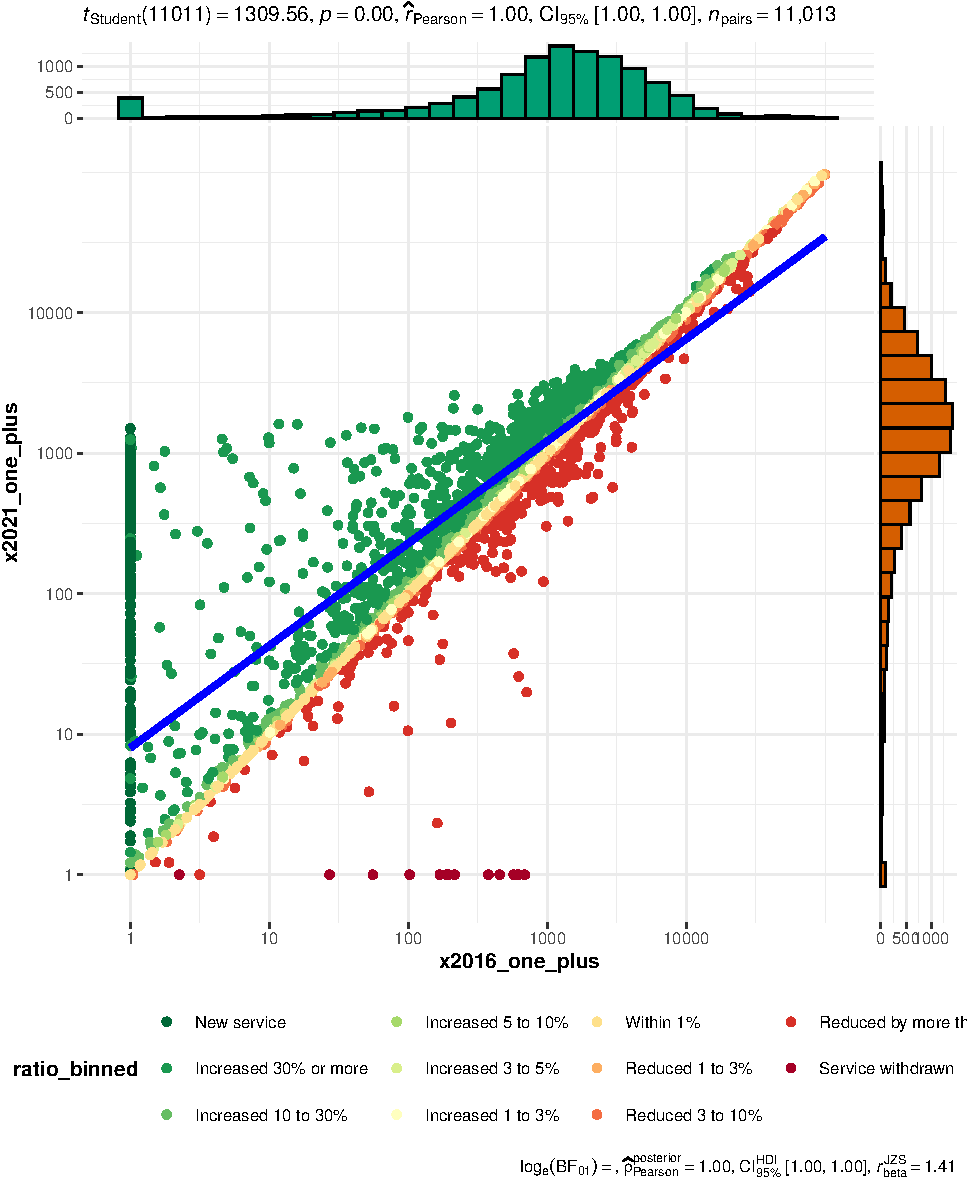
\includegraphics{Leveraging_GTFS_to_assess_transit_supply_Transport_Geography_files/figure-latex/Greater_Melbourne_2016_2021_scatterplot_SA12021-1.pdf}
\caption{Greater Melbourne: SI scores in 2016 and 2021 by SA1 (2021
boundaries), adjusted to set those \textless1 equal to 1 (for visual
clarity)}
\end{figure}

\begingroup\fontsize{8}{10}\selectfont

\begin{longtable}[t]{>{\raggedright\arraybackslash}p{1.75cm}>{\raggedleft\arraybackslash}p{1cm}>{\raggedleft\arraybackslash}p{1cm}>{\raggedleft\arraybackslash}p{1cm}>{\raggedleft\arraybackslash}p{1cm}>{\raggedleft\arraybackslash}p{1cm}>{\raggedleft\arraybackslash}p{1cm}>{\raggedleft\arraybackslash}p{1cm}>{\raggedright\arraybackslash}p{1cm}>{\raggedleft\arraybackslash}p{1cm}>{\raggedleft\arraybackslash}p{1.25cm}}
\caption{\label{tab:Greater_Melbourne_2016_2021_ratio_population_table}Greater Melbourne: Share of 2021 population living in SA1s by change in transit service (2016 vs 2021) by SA4 region}\\
\toprule
Change & Inner & Inner East & Inner South & North East & North West & Outer East & South East & West & M'ton P'sula & Total\\
\midrule
Never served & 0.0\%       (0) & 0.3\%     (478) & 0.9\%   (1,655) & 13.7\%  (24,786) & 12.0\%  (21,762) & 7.1\%  (12,855) & 29.1\%  (52,606) & 23.7\%  (42,883) & 13.2\%  (23,958) & 100.0\%   (180,983)\\
New service & 0.0\%       (0) & 0.0\%       (0) & 0.0\%       (0) & 6.9\%   (9,911) & 25.6\%  (36,817) & 0.2\%     (238) & 37.0\%  (53,254) & 28.2\%  (40,483) & 2.1\%   (3,038) & 100.0\%   (143,741)\\
Increased 30\% or more & 0.4\%   (1,843) & 0.1\%     (279) & 7.6\%  (37,932) & 9.3\%  (46,448) & 16.7\%  (83,007) & 0.8\%   (4,209) & 25.6\% (127,248) & 26.4\% (131,194) & 13.2\%  (65,724) & 100.0\%   (497,884)\\
Increased 10 to 30\% & 11.0\%  (45,197) & 0.8\%   (3,190) & 10.1\%  (41,577) & 10.0\%  (40,989) & 13.7\%  (56,013) & 5.5\%  (22,609) & 18.9\%  (77,391) & 24.8\% (101,767) & 5.1\%  (21,060) & 100.0\%   (409,793)\\
Increased 5 to 10\% & 18.2\%  (72,360) & 3.3\%  (13,018) & 13.1\%  (52,033) & 9.4\%  (37,258) & 7.9\%  (31,400) & 6.7\%  (26,666) & 13.4\%  (53,370) & 25.6\% (101,769) & 2.5\%  (10,149) & 100.0\%   (398,023)\\
\addlinespace
Increased 3 to 5\% & 18.7\%  (79,047) & 5.9\%  (25,074) & 7.2\%  (30,595) & 14.3\%  (60,661) & 13.1\%  (55,445) & 5.6\%  (23,819) & 10.8\%  (45,773) & 20.9\%  (88,601) & 3.5\%  (14,666) & 100.0\%   (423,681)\\
Increased 1 to 3\% & 17.9\% (115,203) & 10.4\%  (67,357) & 9.4\%  (60,889) & 14.4\%  (92,896) & 6.6\%  (42,761) & 6.1\%  (39,263) & 11.7\%  (75,676) & 18.3\% (117,967) & 5.1\%  (32,811) & 100.0\%   (644,823)\\
Within 1\% & 9.2\% (128,666) & 13.5\% (187,974) & 7.0\%  (97,037) & 9.0\% (124,942) & 4.2\%  (57,899) & 19.7\% (274,423) & 19.1\% (266,787) & 10.5\% (146,702) & 7.8\% (109,151) & 100.0\% (1,393,581)\\
Reduced 1 to 3\% & 18.0\%  (49,729) & 14.4\%  (39,675) & 9.9\%  (27,179) & 12.4\%  (34,180) & 5.1\%  (13,986) & 14.1\%  (38,826) & 12.4\%  (34,125) & 7.1\%  (19,517) & 6.7\%  (18,446) & 100.0\%   (275,663)\\
Reduced 3 to 10\% & 27.8\%  (89,662) & 8.0\%  (25,930) & 13.2\%  (42,701) & 13.7\%  (44,261) & 3.5\%  (11,175) & 13.4\%  (43,143) & 7.7\%  (24,903) & 10.3\%  (33,329) & 2.5\%   (7,953) & 100.0\%   (323,057)\\
\addlinespace
Reduced by more than 10\% & 16.0\%  (35,224) & 4.8\%  (10,491) & 14.1\%  (30,989) & 10.3\%  (22,617) & 6.2\%  (13,678) & 14.1\%  (31,042) & 21.6\%  (47,588) & 12.6\%  (27,701) & 0.6\%   (1,228) & 100.0\%   (220,558)\\
Service withdrawn & 0.0\%       (0) & 0.0\%       (0) & 0.0\%       (0) & 30.4\%   (1,777) & 7.3\%     (424) & 21.7\%   (1,270) & 23.3\%   (1,360) & 17.4\%   (1,015) & 0.0\%       (0) & 100.0\%     (5,846)\\
Total & 12.5\% (616,931) & 7.6\% (373,466) & 8.6\% (422,587) & 11.0\% (540,726) & 8.6\% (424,367) & 10.5\% (518,363) & 17.5\% (860,081) & 17.3\% (852,928) & 6.3\% (308,184) & 100.0\% (4,917,633)\\
\bottomrule
\end{longtable}
\endgroup{}

\begin{figure}
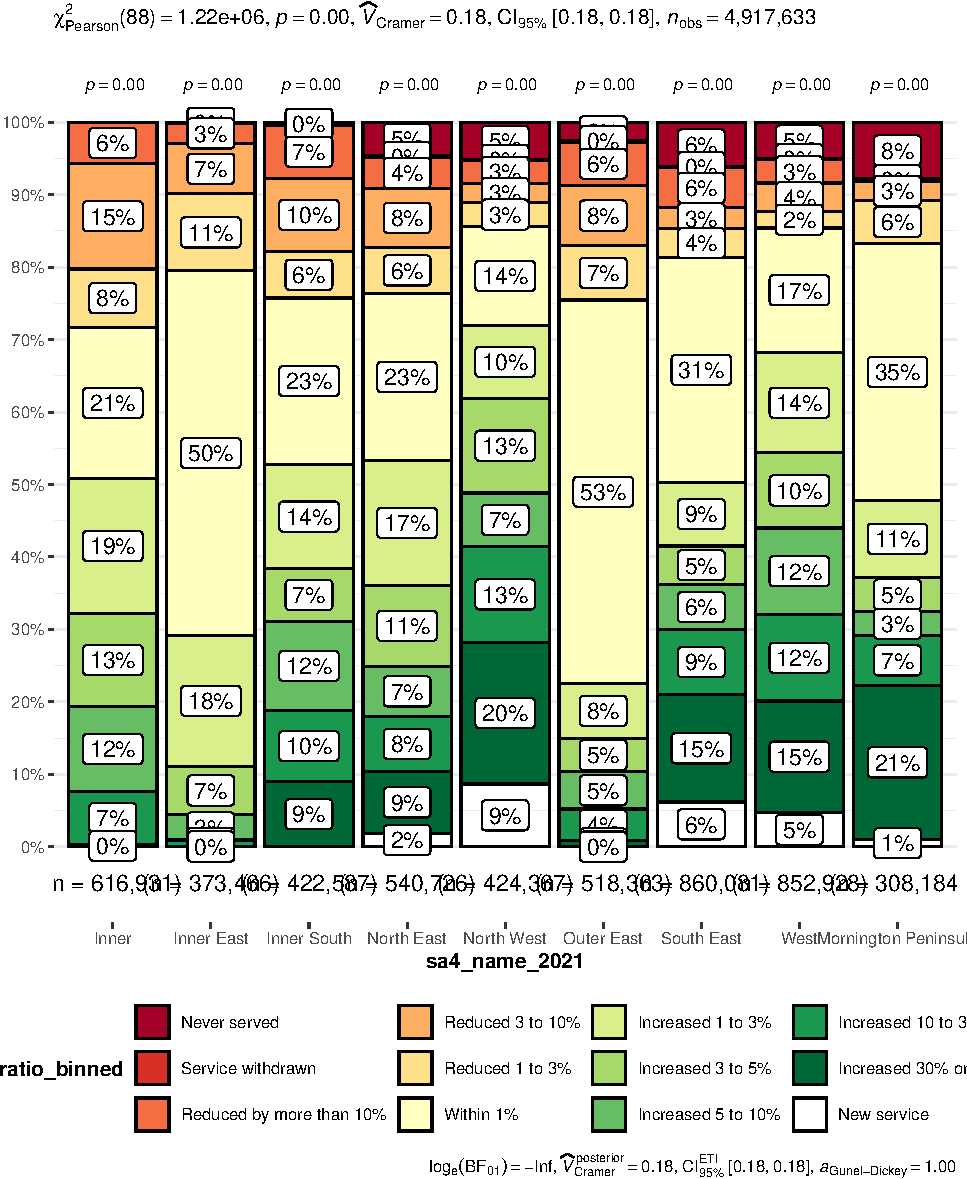
\includegraphics[width=0.9\linewidth]{Leveraging_GTFS_to_assess_transit_supply_Transport_Geography_files/figure-latex/Greater_Melbourne_2016_2021_ratio_population_table-1} \caption{Greater Melbourne: changes in SI between 2016 and 2021, Population by SA4}\label{fig:Greater_Melbourne_2016_2021_ratio_population_table}
\end{figure}

Figure \ref{fig:Greater_Melbourne_2016_2021_scatterplot_SA12021}
compares SI scores across Greater Melbourne (2021 SA1 boundaries) for
2016 and 2021. There is a significant and strong correlation between the
2016 and 2021 SI scores (\(r(11485) = 1.00\), \(p < .001\)). The average
SI score for SA1s across Greater Melbourne increased from 2,843.8 in
2016 to 2,901.4 in 2021 (+2.0\%).

Table \ref{tab:Greater_Melbourne_2016_2021_ratio_population_table}
summarises changes in SI score between 2016 and 2021 (column 1) by SA1s
for the 2021 population, summarised for each SA4 zone (columns 2 to 10)
and Greater Melbourne as a whole (column 11).

\begin{figure}
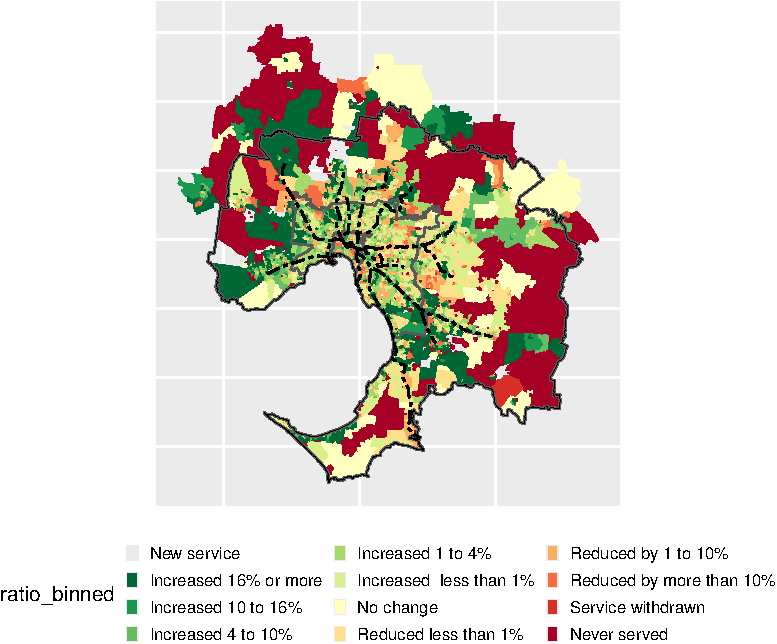
\includegraphics[width=0.9\linewidth]{Leveraging_GTFS_to_assess_transit_supply_Transport_Geography_files/figure-latex/Greater_Melbourne_2016_2021_ratio_map-1} \caption{Greater Melbourne: changes in SI between 2016 and 2021, by SA1}\label{fig:Greater_Melbourne_2016_2021_ratio_map}
\end{figure}

\begin{figure}
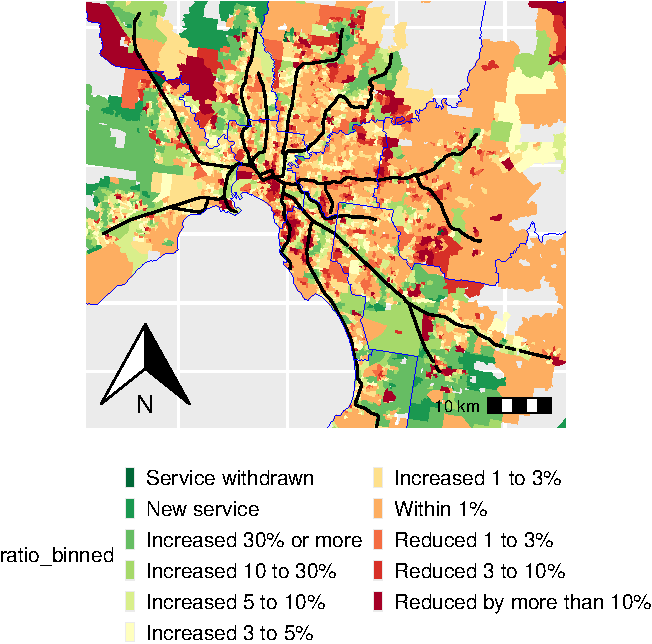
\includegraphics[width=0.9\linewidth]{Leveraging_GTFS_to_assess_transit_supply_Transport_Geography_files/figure-latex/Greater_Melbourne_2016_2021_ratio_map_suburban_railway_extents-1} \caption{Greater Melbourne: changes in SI between 2016 and 2021, by SA1}\label{fig:Greater_Melbourne_2016_2021_ratio_map_suburban_railway_extents}
\end{figure}

Figures \ref{fig:Greater_Melbourne_2016_2021_ratio_map} and
\ref{fig:Greater_Melbourne_2016_2021_ratio_map_suburban_railway_extents}
map the changes in transit service levels between 2016 and 2021. Areas
that have seen service increases include: around the Dandenong,
Cranbourne, Nar Nar Goon, Garfield and Bunyip areas (outer south-east);
some parts of the Mornington Peninsula; Kinglake (outer north-east); and
around Wallan (outer north). Decreased service levels, in contrast are
also evident: along the Stoney Point Line and Koo Wee Rup (outer
south-east); Heathcote Junction (north of Wallan); and around Taylors
Lakes and Syndenham.

---\textgreater{}

\hypertarget{social-needs}{%
\subsubsection{Social needs}\label{social-needs}}

Figure \ref{fig:Greater_Melbourne_2021_social_needs} shows the
distribution of categories of social need index scores across Greater
Melbourne for 2021. This figure is analogous to the 2006 value from
\citet{currie2010identifying} shown in Figure \ref{fig:Currie_map_needs}
although, as discussed in the methodology section above, it was not
possible to exactly replicate the \citet{currie2010identifying} approach
due to changes in the way census results are reported.

\begin{figure}
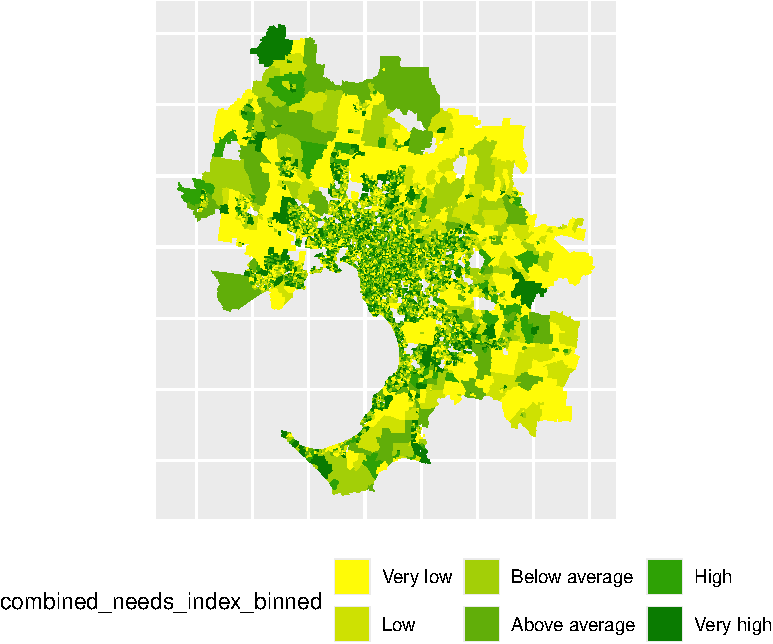
\includegraphics[width=0.9\linewidth]{Leveraging_GTFS_to_assess_transit_supply_Transport_Geography_files/figure-latex/Greater_Melbourne_2021_social_needs-1} \caption{Distribution of categories of composite social need index scores, overlayed with: 2006 Greater Melbourne boundary (black); middle/outer and inner/middle suburb boundaries (grey); and suburban railway lines (dashed).}\label{fig:Greater_Melbourne_2021_social_needs}
\end{figure}

Comparing Figure \ref{fig:Greater_Melbourne_2021_social_needs} and
Figure \ref{fig:Currie_map_needs} suggests that in 2021, compared to
2006:

\begin{itemize}
\tightlist
\item
  the spatial grouping of different levels of social need is less
  consistent, although this may be an artefact of the shift to SA1s from
  CCDs\footnote{CCDs were originally devised to group the approximately
    200 dwellings allocated to each individual census collector, whereas
    SA1s were introduced in be consistent in population (200 to 800
    people, averaging 400) and character\citep{ABS_SA1s_CCDs}}.;
\item
  Lower relative social needs through some parts of the middle northern
  suburbs (around Fawkner and Thornbury), and in the south-east (around
  Dandenong and Lang Lang)
\item
  higher relative needs in some areas of the south-west (around
  Werribee), the northeast (HUrstbridge, Plenty, Bundoora and
  surrounds); and the east (near Gembrook, Maryknoll, and some areas
  around Officer, Beaconsfield and Carrum Downs).
\end{itemize}

\begin{figure}
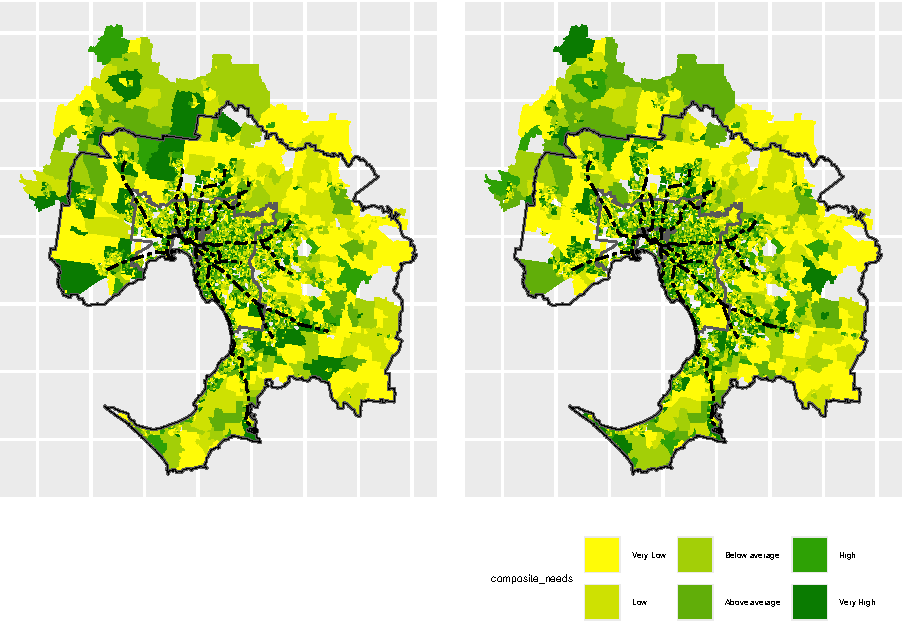
\includegraphics[width=0.9\linewidth]{Leveraging_GTFS_to_assess_transit_supply_Transport_Geography_files/figure-latex/Greater_Melbourne_2016_social_needs-1} \caption{Distribution of categories of composite social need index scores in 2016 (left) and 2021 (right), overlayed with: 2006 Greater Melbourne boundary (black); middle/outer and inner/middle suburb boundaries (grey); and suburban railway lines (dashed).}\label{fig:Greater_Melbourne_2016_social_needs}
\end{figure}

Figure \ref{fig:Greater_Melbourne_2016_social_needs} compares the
spatial patterns of social needs in 2016 and 2021. Overall, the spatial
patterns appear similar, with some areas in the north-west (Gisborne)
and south-east (Carrum Downs, Stoney Point) having Very High needs in
both. Some caution may be required in making direct comparisons of many
outer suburbs where residential development has led to the introduction
of new SA1s for the 2021 census. In many areas, including in the
south-west (Werribee), north-west (Romsey), north (Wallan, Beveridge,
Mickleham) and south-east (Clyde North and Beaconsfield South), it
appears there are still Very High transport needs but the spatial area
covered on the map is much smaller due to the redistricting of larger
SA1s into multiple SA1s. That said, it appears that:

\begin{itemize}
\tightlist
\item
  social needs fell in the southern parts of Bacchus Marsh and areas
  around Melton (outer west);
\item
  social needs rose in some outer northern (Lancefield), eastern
  (Gembrook East) and southern (end of the Mornington Penninsula) areas.
\end{itemize}

\hypertarget{needs-gap-analysis}{%
\subsubsection{Needs-gap analysis}\label{needs-gap-analysis}}

\begingroup\fontsize{7}{9}\selectfont

\begin{longtable}[t]{lrrrrrrr}
\caption{\label{tab:Greater_Melbourne_2021_needs_gap_zones}Greater Melbourne 2021, SA1s within each SI and Combined Needs Index grouping}\\
\toprule
\multicolumn{1}{c}{ } & \multicolumn{6}{c}{Combined Needs Index Category} & \multicolumn{1}{c}{ } \\
\cmidrule(l{3pt}r{3pt}){2-7}
Supply & Very High & High & Above Average & Below Average & Low & Very Low & Total\\
\midrule
Zero Supply & 0.5\%    (61) & 0.5\%    (51) & 0.4\%    (49) & 0.7\%    (79) & 0.9\%    (95) & 1.2\%   (130) & 4.2\%    (465)\\
Very Low & 3.7\%   (408) & 3.3\%   (369) & 3.2\%   (352) & 4.0\%   (444) & 4.1\%   (452) & 4.7\%   (521) & 22.9\%  (2,546)\\
Low & 3.1\%   (346) & 3.4\%   (376) & 3.6\%   (403) & 4.5\%   (500) & 4.6\%   (514) & 4.3\%   (479) & 23.5\%  (2,618)\\
Below average & 3.1\%   (349) & 3.7\%   (412) & 3.9\%   (430) & 4.4\%   (488) & 4.3\%   (482) & 4.3\%   (483) & 23.7\%  (2,644)\\
Above average & 1.4\%   (154) & 1.4\%   (152) & 1.4\%   (157) & 1.7\%   (188) & 1.5\%   (165) & 1.3\%   (140) & 8.6\%    (956)\\
\addlinespace
High & 1.5\%   (165) & 1.5\%   (162) & 1.4\%   (154) & 1.7\%   (193) & 1.5\%   (162) & 1.1\%   (120) & 8.6\%    (956)\\
Very High & 1.7\%   (194) & 1.4\%   (155) & 1.2\%   (133) & 1.3\%   (143) & 1.5\%   (165) & 1.5\%   (163) & 8.6\%    (953)\\
Total & 15.1\% (1,677) & 15.1\% (1,677) & 15.1\% (1,678) & 18.3\% (2,035) & 18.3\% (2,035) & 18.3\% (2,036) & 100.0\% (11,138)\\
\bottomrule
\end{longtable}
\endgroup{}

There is a significant, but only weakly positive correlation between the
2021 SI and Combined Needs Index scores (\(r(11136) = .06\),
\(p < .001\)). Table \ref{tab:Greater_Melbourne_2021_needs_gap_zones}
compares the Transport Supply and Composite Needs groupings for 2021.
Differences in the share of groupings across categories is statistically
significant (\(\chi^2(30, N = 11138) = 133.51\), \(p < .001\)), with
more of the SA1s with higher needs tending to have transport supplies
that are higher than the average. 469 SA1s have Zero or Very Low
transport supply, but very high social needs. This represents 4.2\% of
the 11,138 SA1s within Greater Melbourne, and is a lower proportion than
that reported for 2006 (279 of 5,720 CCDs (4.9\%)) in
\citet{currie2010identifying}.

\begingroup\fontsize{6}{8}\selectfont

\begin{longtable}[t]{lrrrlrrr}
\caption{\label{tab:Greater_Melbourne_2021_needs_gap_population}Greater Melbourne 2021, Population in each SI and Combined Needs Index grouping}\\
\toprule
\multicolumn{1}{c}{ } & \multicolumn{6}{c}{Combined Needs Index Category} & \multicolumn{1}{c}{ } \\
\cmidrule(l{3pt}r{3pt}){2-7}
Supply & Very High & High & Above Average & Below Average & Low & Very Low & Total\\
\midrule
Zero Supply & 0.9\%    (41,915) & 0.6\%  (27,179) & 0.5\%  (22,705) & 0.7\%  (32,328) & 0.7\%  (32,645) & 0.6\%  (30,002) & 3.8\%   (186,774)\\
Very Low & 6.0\%   (291,972) & 4.1\% (199,467) & 3.4\% (165,968) & 3.7\% (182,624) & 3.2\% (158,222) & 2.6\% (129,608) & 23.0\% (1,127,861)\\
Low & 4.9\%   (239,199) & 4.2\% (205,465) & 3.9\% (193,243) & 4.3\% (210,576) & 3.7\% (183,333) & 2.7\% (130,779) & 23.7\% (1,162,595)\\
Below average & 4.7\%   (228,646) & 4.5\% (219,310) & 4.2\% (204,049) & 4.2\% (203,750) & 3.5\% (171,997) & 2.7\% (130,322) & 23.6\% (1,158,074)\\
Above average & 2.0\%   (100,326) & 1.6\%  (80,404) & 1.5\%  (73,669) & 1.6\%  (76,179) & 1.2\%  (56,902) & 0.8\%  (37,419) & 8.7\%   (424,899)\\
\addlinespace
High & 2.2\%   (107,121) & 1.7\%  (83,970) & 1.4\%  (70,132) & 1.6\%  (77,358) & 1.1\%  (54,528) & 0.7\%  (32,274) & 8.7\%   (425,383)\\
Very High & 2.6\%   (129,759) & 1.6\%  (79,306) & 1.2\%  (59,356) & 1.1\%  (55,828) & 1.1\%  (54,061) & 0.8\%  (40,417) & 8.5\%   (418,727)\\
Total & 23.2\% (1,138,938) & 18.3\% (895,101) & 16.1\% (789,122) & 17.1\% (838,643) & 14.5\% (711,688) & 10.8\% (530,821) & 100.0\% (4,904,313)\\
\bottomrule
\end{longtable}
\endgroup{}

\begin{figure}
\centering
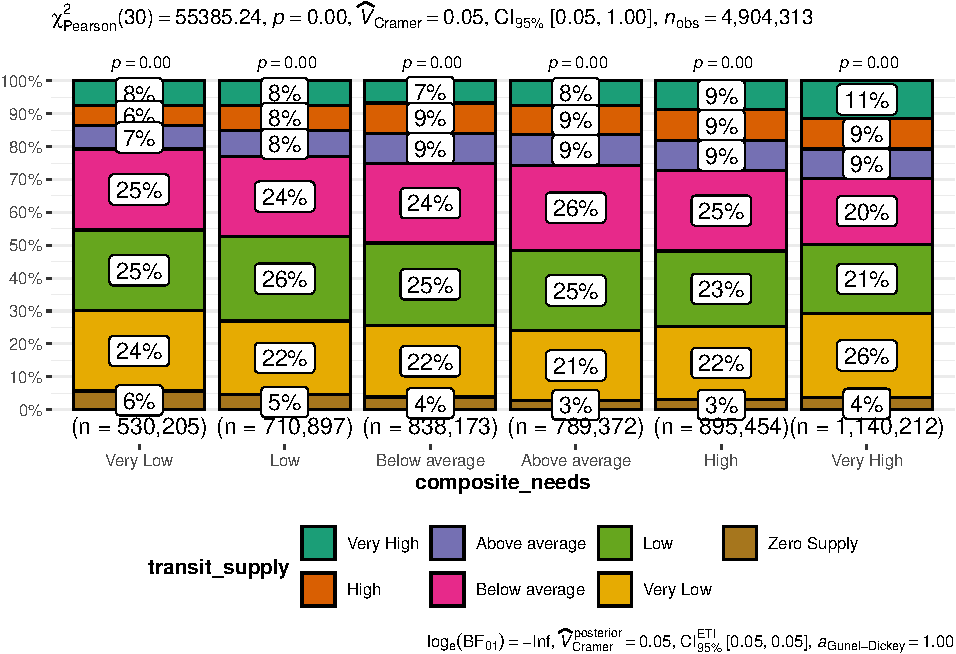
\includegraphics{Leveraging_GTFS_to_assess_transit_supply_Transport_Geography_files/figure-latex/Greater_Melbourne_2021_needs_gap_population-1.pdf}
\caption{Greater Melbourne 2021, Populations within each SI and Combined
Needs Index grouping}
\end{figure}

Table \ref{tab:Greater_Melbourne_2021_needs_gap_population} compares the
populations within each SI and Combined Needs Index grouping for 2021.
There is a statistically significant relationship
(\(\chi^2(30, N = 4904313) = 55715.62\), \(p < .001\)), with more of the
population that has higher needs tending to be living in SA1s that have
transport supplies that ave higher than the average. 333,887 people live
within SA1s that have Zero or Very Low transport supply, but Very High
social needs. This represents 6.8\% of the 4,904,313 people within
Greater Melbourne, and is higher proportion than that reported for 2006
(139,004 of 3.3 million people (4.2\%)).

\begin{figure}
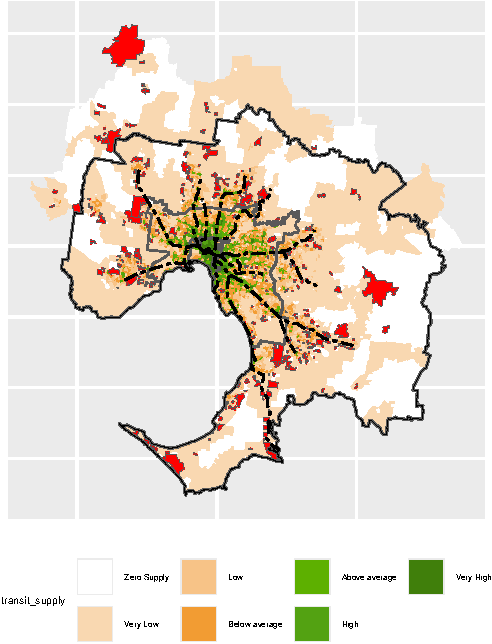
\includegraphics[width=1\linewidth]{Leveraging_GTFS_to_assess_transit_supply_Transport_Geography_files/figure-latex/Greater_Melbourne_2021_needs_gap_map-1} \caption{Greater Melbourne 2021 SI groupings, overlayed with SA1s with very high transport need areas with zero or very low public transport supply (red).}\label{fig:Greater_Melbourne_2021_needs_gap_map}
\end{figure}

Figure \ref{fig:Greater_Melbourne_2021_needs_gap_map} shows SA1 zones in
Greater Melbourne with Very High transport needs, but Very Low or Zero
transit supply for 2021. Comparison to the 2006 spatial distribution
shown in Figure \ref{fig:Currie_map_gap} suggests that:

\begin{itemize}
\tightlist
\item
  areas of the outer west (south west of Sunshine), middle north
  (Broadmeadows), the north-east (Healesville, Powelltown, Yarra
  Junction, Warburton) and the south east (Bunyip, Garfield, Koo Wee
  Rup, Lang Lang) no longer have as large a gap between the social need
  for transport and the level of transit supplied;
\item
  some on the Mornington Penninsula still have gaps, including around
  Stoney Point, Portsa, Blairgowrie and St Andrews Beach; and
\item
  there are many areas, mostly in outer surburbs, that now have large
  gaps between the social need for transport and the level of transit
  provided.
\end{itemize}

\begin{figure}
\centering
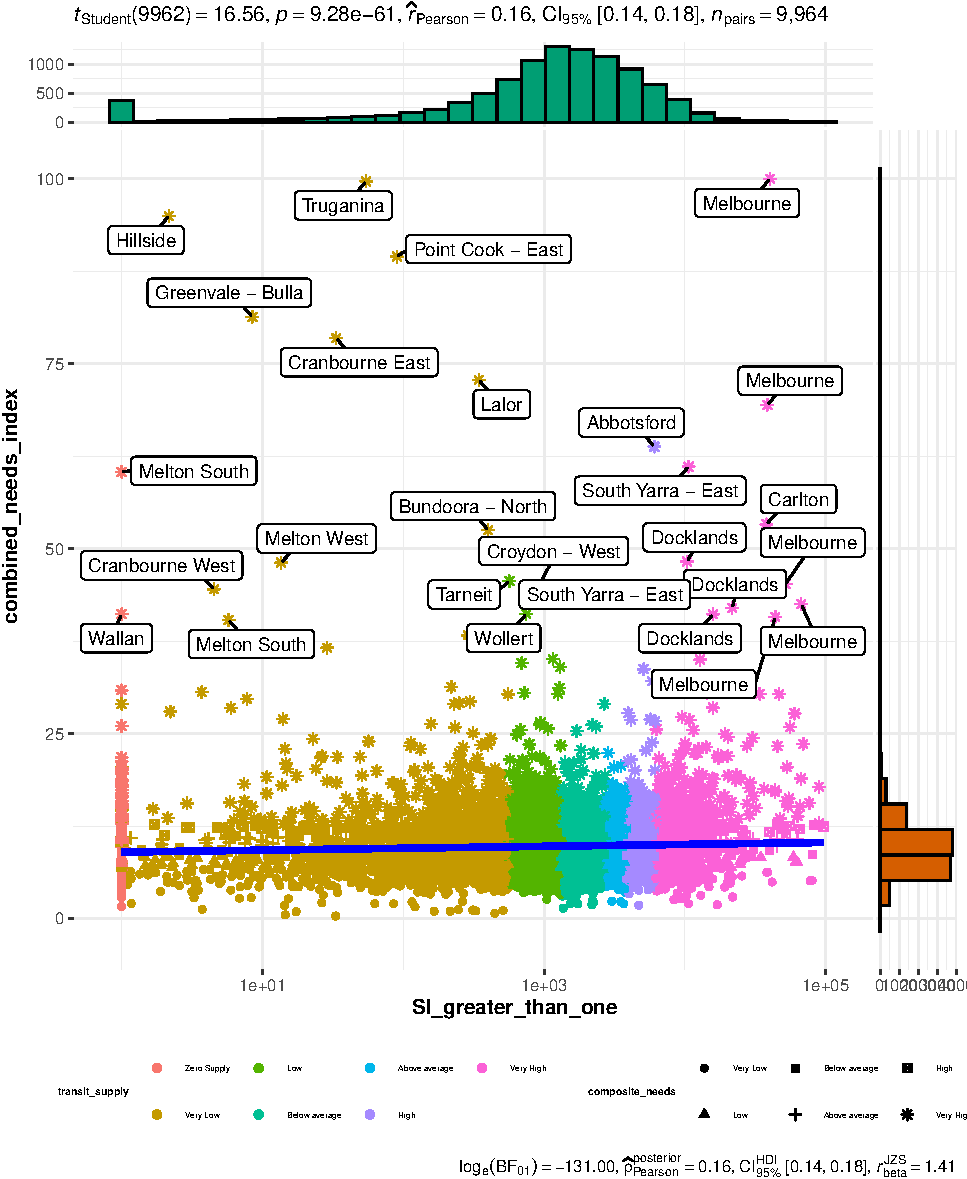
\includegraphics{Leveraging_GTFS_to_assess_transit_supply_Transport_Geography_files/figure-latex/Greater_Melbourne_2016_needs_gap-1.pdf}
\caption{Greater Melbourne 2016, SI and Combined Needs Index scores,
with SI scores \textless{} 1 rounded up to equal 1.}
\end{figure}

Figure \ref{fig:Greater_Melbourne_2016_needs_gap} compares SI and
Combined Needs Index scores for SA1s in 2016. There is a significant,
but only weakly positive relationship.

\begingroup\fontsize{7}{9}\selectfont

\begin{longtable}[t]{lrrrrrrr}
\caption{\label{tab:Greater_Melbourne_2016_needs_gap_zones}Greater Melbourne 2016, SA1s within each SI and Combined Needs Index grouping}\\
\toprule
transit\_supply & Very Low & Low & Below average & Above average & High & Very High & Total\\
\midrule
Zero Supply & 4.8\%    (91) & 3.5\%    (66) & 2.5\%    (47) & 2.4\%    (34) & 2.0\%    (28) & 3.2\%    (46) & 3.1\%   (312)\\
Very Low & 26.1\%   (497) & 23.2\%   (442) & 20.9\%   (397) & 20.4\%   (290) & 19.8\%   (281) & 22.5\%   (319) & 22.3\% (2,226)\\
Low & 24.1\%   (458) & 24.5\%   (467) & 24.4\%   (464) & 22.3\%   (317) & 21.7\%   (308) & 19.7\%   (279) & 23.0\% (2,293)\\
Below average & 24.9\%   (473) & 24.5\%   (467) & 24.1\%   (459) & 23.8\%   (338) & 23.2\%   (329) & 17.6\%   (249) & 23.2\% (2,315)\\
Above average & 7.4\%   (140) & 9.2\%   (175) & 10.2\%   (194) & 10.5\%   (149) & 10.6\%   (150) & 9.2\%   (131) & 9.4\%   (939)\\
\addlinespace
High & 6.5\%   (123) & 7.5\%   (142) & 10.7\%   (203) & 10.2\%   (145) & 12.0\%   (170) & 10.9\%   (155) & 9.4\%   (938)\\
Very High & 6.4\%   (121) & 7.6\%   (144) & 7.3\%   (139) & 10.3\%   (146) & 10.7\%   (152) & 16.9\%   (239) & 9.4\%   (941)\\
Total & 100.0\% (1,903) & 100.0\% (1,903) & 100.0\% (1,903) & 100.0\% (1,419) & 100.0\% (1,418) & 100.0\% (1,418) & 100.0\% (9,964)\\
\bottomrule
\end{longtable}
\endgroup{}

\begin{figure}
\centering
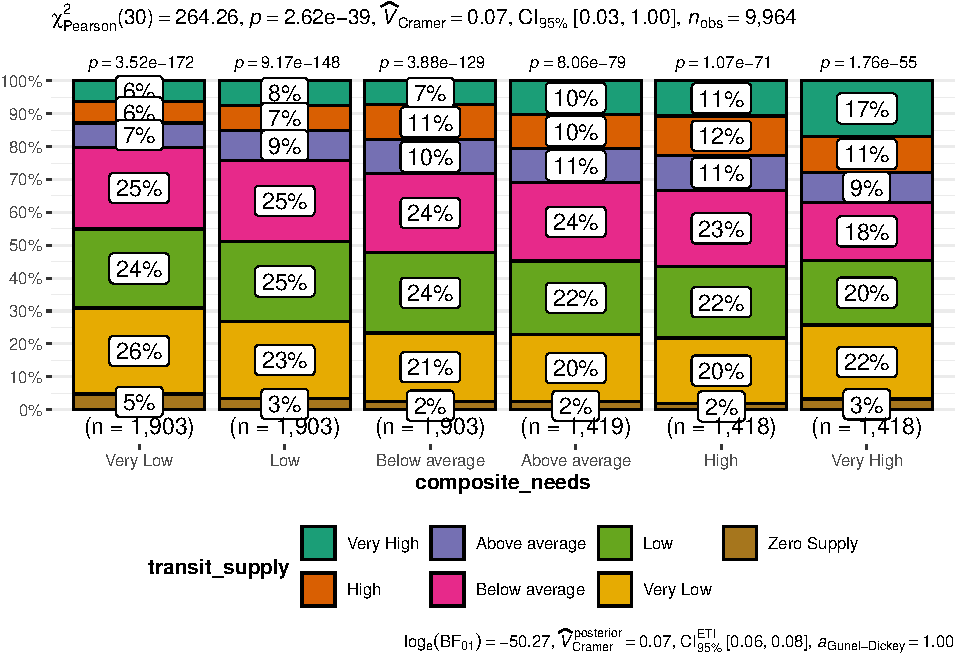
\includegraphics{Leveraging_GTFS_to_assess_transit_supply_Transport_Geography_files/figure-latex/Greater_Melbourne_2016_needs_gap_zones-1.pdf}
\caption{Greater Melbourne 2016, SA1s within each SI and Combined Needs
Index grouping}
\end{figure}

Figure \ref{fig:Greater_Melbourne_2016_needs_gap_zones} and Table
\ref{tab:Greater_Melbourne_2016_needs_gap_zones} compares the SI and
Combined Needs Index groupings for 2016. There is a statistically
significant relationship, although this appears to be weak. 365 SA1s
have zero or very low transit supply, but very high social needs. This
represents 3.7\% of the 9,964 SA1s within Greater Melbourne, and is a
higher proportion than that reported for 2006 (85 of 5,720 CCDs
(1.6\%)).

\begingroup\fontsize{7}{9}\selectfont

\begin{longtable}[t]{>{\raggedright\arraybackslash}p{2cm}>{\raggedleft\arraybackslash}p{1.16cm}>{\raggedleft\arraybackslash}p{1.16cm}>{\raggedleft\arraybackslash}p{1.16cm}>{\raggedleft\arraybackslash}p{1.16cm}>{\raggedleft\arraybackslash}p{1.16cm}>{\raggedleft\arraybackslash}p{1.16cm}>{\raggedleft\arraybackslash}p{1.5cm}}
\caption{\label{tab:Greater_Melbourne_2016_needs_gap_population}Greater Melbourne 2016, Population in each SI and Combined Needs Index grouping}\\
\toprule
transit\_supply & Very Low & Low & Below average & Above average & High & Very High & Total\\
\midrule
Zero Supply & 4.3\%  (22,012) & 3.3\%  (22,544) & 2.4\%  (18,784) & 2.3\%  (15,402) & 1.9\%  (14,790) & 3.6\%    (38,050) & 2.9\%   (131,582)\\
Very Low & 24.8\% (126,298) & 23.1\% (156,359) & 20.8\% (165,350) & 20.5\% (138,710) & 20.1\% (153,169) & 25.1\%   (263,693) & 22.4\% (1,003,579)\\
Low & 24.8\% (126,411) & 24.9\% (168,228) & 24.8\% (197,542) & 22.8\% (154,275) & 22.1\% (168,541) & 19.1\%   (200,937) & 22.7\% (1,015,934)\\
Below average & 25.4\% (129,440) & 25.1\% (169,849) & 24.4\% (193,915) & 24.1\% (163,593) & 23.2\% (177,044) & 15.7\%   (164,681) & 22.3\%   (998,522)\\
Above average & 7.5\%  (38,003) & 9.1\%  (61,679) & 10.1\%  (80,591) & 10.3\%  (70,066) & 10.5\%  (80,172) & 8.1\%    (84,562) & 9.3\%   (415,073)\\
\addlinespace
High & 6.6\%  (33,334) & 7.3\%  (49,615) & 10.4\%  (83,055) & 9.9\%  (67,061) & 11.7\%  (89,517) & 10.1\%   (105,960) & 9.6\%   (428,542)\\
Very High & 6.6\%  (33,361) & 7.2\%  (48,441) & 7.1\%  (56,303) & 10.1\%  (68,467) & 10.4\%  (79,329) & 18.3\%   (192,038) & 10.7\%   (477,939)\\
Total & 100.0\% (508,859) & 100.0\% (676,715) & 100.0\% (795,540) & 100.0\% (677,574) & 100.0\% (762,562) & 100.0\% (1,049,921) & 100.0\% (4,471,171)\\
\bottomrule
\end{longtable}
\endgroup{}

\begin{figure}
\centering
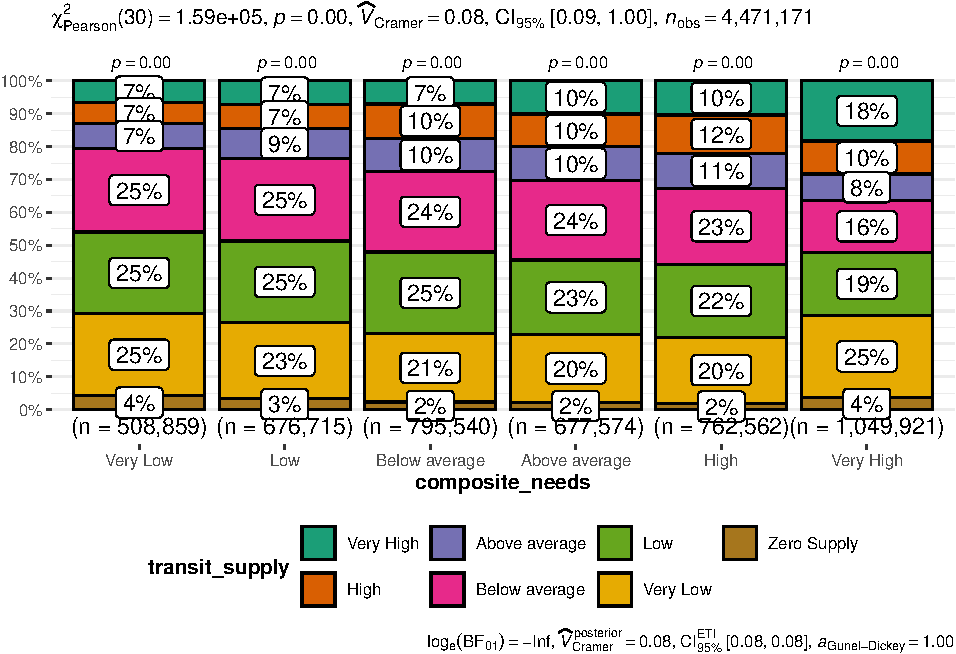
\includegraphics{Leveraging_GTFS_to_assess_transit_supply_Transport_Geography_files/figure-latex/Greater_Melbourne_2016_needs_gap_population-1.pdf}
\caption{Greater Melbourne 2016, Populations within each SI and Combined
Needs Index grouping}
\end{figure}

Figure \ref{fig:Greater_Melbourne_2016_needs_gap_population} and Table
\ref{tab:Greater_Melbourne_2016_needs_gap_population} compares the
populations within each SI and Combined Needs Index grouping for 2016.
There is a statistically significant relationship, although this appears
to be weak. 301743 people live within SA1s that have zero or very low
transit supply, but very high social needs. This represents 6.7\% of the
4,471,171 people within Greater Melbourne, and is a lower proportion
than that reported for 2006 (37,699 of 3.3 million people (8.2\%)).

Figure \ref{fig:Greater_Melbourne_2016_needs_gap_map} shows SA1 zones in
Greater Melbourne with Very High transport needs, but Very Low or Zero
transit supply for 2016 (left) and 2021 (right) in red. There are no
SA1s within the inner suburbs with Very High transport needs, but Very
Low or Zero transit supply in either 2016 or 2021. In the middle suburbs
there appear to be some minor shifts, but the overall pattern in both
2016 and 2021 appears to be that there are isolated areas of Very High
transport needs, but Very Low or Zero transit supply in between train
lines. In the outer suburbs, however:

\begin{itemize}
\tightlist
\item
  areas around Werribee (south-west) continue to have Very High
  transport needs, but Very Low or Zero transit supply, and many of the
  changes between 2016 and 2021 appear to be related to new SA1 zones
  being added.
\item
  there appears to have been some improvement around Bacchus Marsh and
  Melton (west), but again, this may be an aterfact of some of the 2016
  SA1 zones having been split in 2021.\\
\item
  no improvements around Gisbourne (west-north-west)
\item
  some shifts around Lancefield and Romsey (north-west), Kilmore and
  west of Craigieburn (north-north-west), but again these may being in
  part due to boundary changes;
\item
  no improvement around Mernda, Diamond Creek and (west of) Hurstbridge
  (north-east) or around the outer eastern or south-eastern suburbs;
\item
  additions in the outter east and south including in parts of the
  Mornington Peninsula (south) and places close to Emerald and Gembrook.
\end{itemize}

\hypertarget{discussion}{%
\section{Discussion}\label{discussion}}

\hypertarget{limitations}{%
\subsection{Limitations}\label{limitations}}

\hypertarget{directions-for-furture-research}{%
\subsection{Directions for furture
research}\label{directions-for-furture-research}}

\hypertarget{conclusions}{%
\section{Conclusions}\label{conclusions}}

\renewcommand\refname{References}
\bibliography{References.bib, packages.bib}


\end{document}
